\documentclass[a4paper,11pt]{scrartcl}

\usepackage[ngerman]{babel}
\usepackage[hidelinks]{hyperref}
\usepackage{apacite}
\usepackage{graphicx}
\usepackage{subcaption}
\usepackage{float}
\usepackage{longtable}
\usepackage{tabularx}
    \usepackage{array}
    \usepackage{multicol}
    \usepackage{multirow}
    \usepackage{makecell}
\usepackage[table]{xcolor}
\usepackage{fontspec}
    \setmainfont{EB Garamond}
    \setsansfont{Open Sans}
    \setmonofont{Fira Mono}[SizeFeatures={Size=8}]
\usepackage{listings}
    \lstset{basicstyle=\footnotesize\ttfamily}
\usepackage{nameref}
\usepackage{rotating}
\usepackage{amsmath}
\usepackage{gensymb}
\usepackage{enumitem}
\usepackage{hyphenat}
\usepackage{metalogo}

\newcommand{\imgref}[1]{{siehe \textit{Abbildung \ref{#1}, Seite \pageref{#1}}}}
\newcommand{\imgrefplain}[1]{{\textit{Abbildung \ref{#1}, Seite \pageref{#1}}}}
\newcommand{\secref}[1]{{siehe \textit{Abschnitt \ref{#1}: \nameref{#1}, Seite \pageref{#1}}}}
\newcommand{\secrefplain}[1]{{\textit{\ref{#1}: \nameref{#1}, Seite \pageref{#1}}}}
\newcommand{\tblref}[1]{{siehe \textit{Tabelle \ref{#1}: \nameref{#1}, Seite \pageref{#1}}}}
\newcommand{\tblrefplain}[1]{{\textit{Tabelle \ref{#1}: \nameref{#1}, Seite \pageref{#1}}}}
\newcommand{\calcref}[1]{{siehe \textit{Berechnung \ref{#1}, Seite \pageref{#1}}}}
\newcommand{\calcrefplain}[1]{{\textit{Formel \ref{#1}, Seite \pageref{#1}}}}
\newcommand{\appref}[1]{\textit{Anhang \ref{#1}: \nameref{#1}}}

\newenvironment{itemizecell}[1]{\begin{tabular}{@{\textbullet~}p{#1}@{}}}{\end{tabular}}

\renewcommand{\baselinestretch}{1.2}
\pagestyle{headings}

\renewcaptionname{ngerman}{\refname}{Quellen}

\begin{document}

\author{PREN Gruppe 7}
\title{Silisloth}
\subtitle{Dokumentation PREN 2}
\date{\today}

\begin{multicols}{2}
\maketitle
\columnbreak
    \includegraphics[width=0.75\columnwidth]{pics/assembly-schraeg.png}
\end{multicols}

\section*{Versionierung}
\def\arraystretch{1.2}
\begin{tabularx}{\textwidth}{|r|l|X|}
\hline
\textbf{Version} & \textbf{Datum} & \textbf{Bemerkung} \\
\hline
0.1 & Fr, 23.03.2018 & Aufsetzen des Dokuments \\
0.2 & Fr, 25.05.2018 & Fertigstellung der Vorabversion \\
1.0 & Fr, 10.06.2018 & Fertigstellung für Schlussabgabe \\
\hline
\end{tabularx}
\vspace{1em}

\begin{multicols}{2}
\section*{Betreuer}
Zeno \textsc{Stössel}, Elektrotechnik
\section*{Experten}
Jörg \textsc{Hofstetter}, Informatik \\
Carsten \textsc{Haak}, Maschinentechnik
\vfill\null
\columnbreak
\section*{Autoren}
Sandro \textsc{Bertozzi}, Informatik \\
Christoph \textsc{Binkert}, Maschinentechnik \\
Patrick \textsc{Bucher}, Informatik \\
Alex \textsc{Duong}, Elektrotechnik \\
Quentin \textsc{Frei}, Maschinentechnik \\
Jan \textsc{Greber}, Elektrotechnik \\
Marko \textsc{Lovrinovic}, Maschinentechnik \\
Johannes \textsc{Togan}, Maschinentechnik
\end{multicols}

\newpage
\section*{Teamvorstellung Gruppe 7}

\begin{figure}[H]
    \centering
    \includegraphics[width=0.9\linewidth]{pics/team.jpg}
    \caption{Gruppenfoto (von links nach rechts): Alex Duong, Christoph Binkert, Sandro Bertozzi, Quentin Frei (vorne), Patrick Bucher (hinten), Jan Greber, Marko Lovrinovic (vorne), Johannes Togan (hinten)}
    \label{fig:team}
\end{figure}

\begin{multicols}{2}
\begin{itemize}
    \item Alex \textsc{Duong} (Elektrotechnik)\\ \href{mailto:alex.duong@stud.hslu.ch}{\texttt{alex.duong@stud.hslu.ch}}
    \item Christoph \textsc{Binkert} (Maschinentechnik)\\ \href{mailto:christoph.binkert@stud.hslu.ch}{\texttt{christoph.binkert@stud.hslu.ch}}
    \item Sandro \textsc{Bertozzi} (Informatik)\\ \href{mailto:sandro.bertozzi@stud.hslu.ch}{\texttt{sandro.bertozzi@stud.hslu.ch}}
    \item Quentin \textsc{Frei} (Maschinentechnik)\\ \href{mailto:quentin.frei@stud.hslu.ch}{\texttt{quentin.frei@stud.hslu.ch}}
\end{itemize}
\columnbreak
\begin{itemize}
    \item Patrick \textsc{Bucher} (Informatik)\\ \href{mailto:patrick.bucher@stud.hslu.ch}{\texttt{patrick.bucher@stud.hslu.ch}}
    \item Jan \textsc{Greber} (Elektrotechnik)\\ \href{mailto:jan.greber@stud.hslu.ch}{\texttt{jan.greber@stud.hslu.ch}}
    \item Marko \textsc{Lovrinovic} (Maschinentechnik)\\ \href{mailto:marko.lovrinovic@stud.hslu.ch}{\texttt{marko.lovrinovic@stud.hslu.ch}}
    \item Johannes \textsc{Togan} (Maschinentechnik)\\ \href{mailto:johannes.togan@stud.hslu.ch}{\texttt{johannes.togan@stud.hslu.ch}}
\end{itemize}
\end{multicols}

\newpage
\section*{Management Summary}

Dieses Dokument wurde im Rahmen des Moduls PREN 2 im Frühlingssemester 2018 von der Gruppe 7 erstellt und dokumentiert die Umsetzung der autonomen Laufkatze \textit{Silisloth}, wie sie im Herbstsemester 2017 im Rahmen des Moduls PREN 1 konzipiert worden ist. \textit{Silisloth} ist ein Gerät, das an einem Seil hängend nach erteiltem Startsignal eine Last lokalisieren, aufnehmen, über Hindernisse hinweg befördern und in einem durch konzentrische Quadrate markierten Zielbereich absetzen kann. Die hier vorliegende Dokumentation beschreibt die Umsetzung der Bereiche Mechanik (Aufbau, Montage), Elektronik (Schaltungen, Verdrahtung, Motorensteuerung), Informatik (Bildverarbeitung, Steuerung, Smartphone-App) wie auch interdisziplinäre Fragestellungen (Kommunikation zwischen den Geräten, vorgenommene Tests) sowie den geplanten Ablauf beim Absolvieren der gestellten Wettbewerbsaufgabe. Wie schon das zugrundeliegende Konzept \cite{pren1}, auf das in diesem Dokument bei Bedarf verwiesen wird, folgt die Umsetzung der Maxime «eine sichere, zuverlässige und für alle verständliche Lösung zu erarbeiten, die dennoch originell und für alle Beteiligten lehrreich ist und zur Zusammenarbeit über die Fachgrenzen hinweg anregt», wie sie in PREN 1 als Gruppenziel formuliert worden ist.

\newpage
\tableofcontents
\newpage
\section{Einleitung}

In PREN 1 wurde das Konzept für \textit{Silisloth} -- eine autonome Laufkatze -- entwickelt. In PREN 2 wurde dieses umgesetzt. Die verwendeten und entwickelten Komponenten und die Konstruktion folgen dabei grösstenteils diesem Konzept. Das vorliegende Dokument gibt einen Überblick über den dabei erstellten Prototypen und handelt von dessen Umsetzung. Änderungen gegenüber dem ursprünglichen Konzept werden dabei gesondert hervorgehoben. Um Wiederholungen und das Kopieren von Passagen zu vermeiden, wird bei Bedarf auf das Konzept \cite{pren1} verwiesen.

Die Konstruktion bildet die Grundlage von \textit{Silisloth}. Die schlanke Lösung, die den Prinzipien der Leichtbauweise folgt, wird in Abschnitt \secrefplain{sec:konstruktion} beschrieben. Eine Explosionsansicht des CAD-Modells bietet einen Überblick über die einzelnen Komponenten und deren Anordnung.

In Abschnitt \secrefplain{sec:elektronik} geht es einerseits um verschiedene Elektrotechnikkomponenten, die im Konzept von PREN 1 noch nicht erwähnt wurden, andererseits um die Verdrahtung der elektronischen Komponenten miteinander. Last- und Steuerstromkreis werden in einem Blockschema dargestellt.

In Abschnitt \secrefplain{sec:ablauf} wird das Absolvieren der Wettbewerbsaufgabe aus einer technischen Perspektive erläutert. Der Leser erhält dadurch einen Einblick in die Funktionsweise von \textit{Silisloth}, und erfährt, welche Überlegungen gemacht wurden, um das gestellte Problem erfolgreich zu lösen. Für Implementierungsdetails wird auf später folgende Abschnitte verwiesen.

\textit{Silisloth} ist mehr als ein elektromechanisches Gerät. Es ist mit einem Raspberry Pi (fortan «Raspi» genannt) und einem Arduino ausgestattet, was schon genügt um es als fahrendes Rechennetzwerk zu bezeichnen. Das Startsignal wird von einer Smartphone-App aus erteilt, welche auch die Lastkoordinaten anzeigt. Ein externer Laptop dient dazu den Ablauf des Raspi-Programms zu überwachen -- und um \textit{Silisloth} in Bereitschaft zu versetzen. Die verschiedenen Kommunikationsprotokolle, die im Zusammenspiel dieser vier Computer zum Einsatz kommen, werden in Abschnitt \secrefplain{sec:kommunikation} beschrieben. Zur Veranschaulichung wird ein UML-Sequenzdiagramm verwendet.

Neben der Kommunikation stellt das Erkennen des Zielfeldes und die Ermittlung des Abstandes zu diesem eine grosse Herausforderungen dar. Der Abschnitt \secrefplain{sec:bildverarbeitung} geht ausführlich auf die erarbeitete Lösung ein. Dabei wird zwar auch die dabei verwendete OpenCV-Library und die Programmiersprache Python angesprochen, die Erläuterungen sollen aber dennoch für einen Leser verständlich sein, der in diesen Technologien nicht bewandert ist. Eine Bildserie des Zielfeldes vermittelt dem Leser die Perspektive der Kamera, was die erstellte Lösung bessser nachvollziehbar macht.

\textit{Silisloth} erfordert zum Betrieb verschiedene Softwarekomponenten. Die Smartphone-App zur Erteilung des Startsignals wird in Abschnitt \secrefplain{sec:smartphoneapp} erläutert. Die ganze Programmlogik, die \textit{Silisloth} zu einem autonomen Gerät machen, ist auf einen Raspi und einen Arduino verteilt. Abschnitt \secrefplain{sec:raspi} geht auf die Python-Lösung ein, welche einerseits die Aktionen von \textit{Silisloth} koordiniert und andererseits verschiedene Hardware- und Kommunikationsschnittstellen bedient. Ein UML-Klassendiagramm verschafft Übersicht über das erstellte Python-Projekt. Der Abschnitt \secrefplain{sec:arduino} handelt von der in C und mit der RTOS-Library geschriebenen Softwarelösung, welche in erster Linie für die Motorensteuerung zuständig ist, jedoch auch Kommunikations- und Koordinationsprobleme löst. Besonders wichtig sind hier interne Stati, welche mit einer State-Machine veranschaulicht werden.

Der in PREN 2 erarbeitete Prototyp soll, wie schon das in PREN 1 erstelle Konzept, den gestellten Anforderungen genügen. Inwiefern diese Anforderungen erfüllt sind, und wie der Prototyp mittels Tests kontinuierlich verbessert wurde, ist Thema von Abschnitt \secrefplain{sec:zielerreichung}.

Im Abschnitt \secrefplain{sec:schlusswort} wird die Umsetzung des \textit{Silisloth}-Projektes reflektiert. Dabei wird einerseits auf die einzelnen Projektphasen in der Umsetzung, andererseits auf bestimmte dabei gemachte Erfahrungen eingegangen. Am Schluss wird ein Fazit gezogen, welches -- soviel vorweg -- aufgrund der gelungenen Lösung positiv ausfällt.

\subsection{Verwendete Werkzeuge}

Die Arbeit wurde mit \LaTeX\footnote{\url{https://www.latex-project.org/}} und \XeLaTeX\footnote{\url{https://www.sharelatex.com/learn/XeLaTeX}} in den Schriftarten EB Garamond, \textsf{Open Sans} und \texttt{Fira Mono} gesetzt. Die Grafiken wurden mit \textit{Graphviz}\footnote{\url{https://www.graphviz.org/}}, \textit{plantuml}\footnote{\url{http://plantuml.com/}} und \textit{LibreOffice Draw}\footnote{\url{https://www.libreoffice.org/discover/draw/}} erstellt. Weitere Hilfsmittel waren \texttt{git}\footnote{\url{https://git-scm.com/}} zur Versionsverwaltung der Quelldateien und \texttt{make}\footnote{\url{https://www.gnu.org/software/make/}} zum Erstellen der Grafiken und des Dokuments aus den Quelldateien.

\newpage
\section{Konstruktion}
\label{sec:konstruktion}

\begin{figure}
    \centering
    \includegraphics[width=1.0\linewidth]{graphs/beschriftung.png}
    \caption{Die Explosionsansicht des CAD-Modells von \textit{Silisloth} mit nummerierten Komponenten}
    \label{fig:explosionsansicht}
\end{figure}

Die Konstruktion von \textit{Silisloth} (\imgref{fig:explosionsansicht}) folgt weitgehend den CAD-Plänen von PREN 1 \cite[S. 12-13]{pren1}. Einige Teile sind dazugekommen (Endschalter, PCB), manche Teile wurden anders positioniert (Ultraschallsensor in x-Richtung, Luftpumpen und Magnetventil) und in manchen Bereichen wurde die Konstruktion verfeinert und optimiert (Greifeinheit, Kontrollbox). Die Konstruktion lässt sich in drei Bereiche unterteilen und besteht aus den folgenden Komponenten:

\begin{multicols}{2}

\textsc{A: Aufhängung}

\begin{enumerate}
    \item Halterungsschiene für Aufhängung
    \item Laufrollen mit Bolzen
    \item Antriebsrad
    \item Quick-Pins zur Befestigung
    \item Riemengetriebe für den Antrieb (Übersetzung)
    \item Getriebemotor für den Antrieb
    \item Endschalter
    \item Bolzen zur Befestigung der Kontrollbox
\end{enumerate}

\textsc{B: Kontrollbox}

\begin{enumerate}
\setcounter{enumi}{8}
    \item LiPo-Akku (Laststromkreis)
    \item Motor Shield
    \item Arduino
    \item LiPo-Akku (Steuerstromkreis) mit USV (verborgen)
    \item Raspberry Pi
    \item Laufrolle für Hubmechanismus
    \item PCB für Ultraschallsensoren
    \item Ultraschallsensor in x-Richtung
    \item Ultraschallsensor in z-Richtung
    \item Raspi-Cam (neigbar)
    \item Seiltrommel
    \item Schrittmotor mit Kühlkörper
    \item Riemengetriebe für den Hubmechanismus (Untersetzung)
    \item Laufrollen für Seilwinde
\end{enumerate}

\textsc{C: Greifmechanismus}

\begin{enumerate}
\setcounter{enumi}{22}
    \item Luftpumpen
    \item Spiralkabel
    \item Magnetventil
    \item Silikongreifer
\end{enumerate}

\end{multicols}

In den folgenden Abschnitten wird erläutert, auf welche Eigenschaften bei der Umsetzung besonderen Wert gelegt wurde, und wie dabei die Designentscheide gefällt wurden.

\subsection{Kontrollbox}

Während der konstruktiven Phase wurde besonderen Wert auf die Designeigenschaften Zugänglichkeit und Kompaktheit gelegt. Es sollte gewährleistet sein jederzeit auf alle Komponenten zugreifen zu können, damit an diesen, wenn nötig, Eingriffe vorgenommen werden können, ohne dass eine Demontage nötig oder Betriebsunterbrüche daraus resultieren würden. Es wurde speziell darauf geachtet Stapelung von Komponenten zu vermeiden.

In Bezug auf die Kompaktheit wurde besonders auf platzsparendes Design, einfache Transportierbarkeit und ein geringes Gewicht geachtet.

Beim Seilwindenmotor war während der Designphase nicht sicher, ob dieser den Anforderungen genügt. Deshalb wurde hier eine Adapterplatte eingesetzt, sodass nur diese Platte und nicht eine ganze Komponente ausgetauscht werden müsste, sollte ein anderer Seilwindenmotor zum Einsatz kommen. Zusätzlich wurde die Adapterplatte mit Langlöchern versehen, womit sich der Achsenabstand leicht variieren lässt. Dies dient einerseits dem Toleranzausgleich und andererseits zum Spannen des Riemens.

Grosser Wert wurde bei der Konstruktion darauf gelegt, dass der Schwerpunkt an der richtigen Stelle zu liegen kommt, sodass der Verbindungsbolzen und der Schwerpunkt der Kontrollbox zusammen mit dem Greifmechanismus im Lot sind. Dies setzte voraus, dass das Einzelgewicht aller Komponenten bekannt bzw. die Dichte aller Materialien hinterlegt war. Deshalb mussten zunächst alle Kaufteile beschafft werden, bevor die Kontrollbox gelasert werden konnte.

Für die finale Justierung wurde die Konstruktion so gewählt, dass der Akku in x-Richtung leicht variabel verbaubar ist, was einen gewissen Korrekturspielraum zulässt.

Dieser Ansatz wurde gewählt, damit für die Sensorikelemente (Ultraschallsensoren) mit einer geringen Toleranzbreite gearbeitet werden konnte. So konnte zusätzlich die Anzahl möglicher Fehl- oder Störquellen bei den Sensoren minimiert werden. Bei der Kamera war der optimale Blickwinkel noch nicht bekannt. Deshalb fiel die Wahl bewusst auf eine einstellbare Halterung, die sich um $75\degree$ an der y-Achse rotieren lässt.

\subsection{Greifmechanismus}

Der Greifmechanismus ist symmetrisch um die x-z-Ebene und die y-z-Ebene aufgebaut. Damit liegt der Schwerpunkt in seinem Zentrum, wodurch gewährtleistet ist, dass der Mechanismus jederzeit horizontal, und der Silikongreifer optimal ausgerichtet ist.

Bei der Konstruktion des Greifmechanismus wurde auf einen kompakten Aufbau geachtet, damit die Perspektive der Kamera möglichst wenig eingeschränkt wird. Auch diese Konstruktion folgt der Leichtbauweise, sodass der Seilwindenmotor mit dem Hubmechanismus nicht am Limit betrieben werden muss.

Um die Stabilität des Greifers zu gewährleisten, wurde eine Halterung konstruiert. Zwei Platten halten den Greifer zusammen. Greifer, Platten, Luftpumpen, Magnetventil, Umlenkrollen und unteres Gerüst bilden den Greifmechanismus.

Der Silikongreifer wird mit zwei $12V$-Luftpumpen aufgeblasen. Bei den ersten Versuchen wurde festgestellt, dass eine Pumpe alleine den Greifer nicht genug schnell mit Luft füllt. Bei zwei Pumpen wurde dann die gewünschte Griff-Geschwindigkeit erreicht.

Damit der Luftstrom gesteuert werden kann, ist ein Magnetventil zwischen Luftpumpen und Silikongreifer geschaltet. Somit kann die Luft zu einem gewünschten Zeitpunkt aus dem Greifer weggeführt werden.

Um die Dichtheit zu testen, wurde der Greifer mit Luft gefüllt und ein Würfel eingeklemmt. Der Greifer hielt den Würfel über vier Minuten in der Luft, somit erfüllte er die Anforderungen. Die Herstellung des Silikongreifers wurde bereits in der Dokumentation von PREN 1 \cite[S. 44-46]{pren1} beschrieben.

\subsection{Weitere Aspekte der Konstruktion}

\begin{description}
    \item[Fortbewegung] Das treibende, sich in der Mitte der Aufhängung befindende Kunststoffrad wird über einen Zahnriemen von einem Getriebemotor angetrieben. Das Antriebsrad befindet sich unterhalb des Stahlseils, damit mehr Normalkraft für die Kraftübertragung (Reibung) gewonnen werden kann. Zwei zusätzliche, nicht angetriebene Kunststoffräder, welche sich oberhalb des Seils befinden, stützen die Laufkatze. Die Räder sind auf Stahlwellen befestigt, welche wiederum in Kugellagern laufen, um einen möglichst geringen Reibungsverlust zu erzielen.
    \item[Berechnung für die Wellenabstände] Die Berechnung für die Wellenabstände, welche für die Aufhängung und Kontrollbox verwendet wird, erfolgt über die \calcrefplain{eq:wellenabstand} \cite[Kapitel 16, Formel 22]{roloff-matek}.
    \item[Polyvalenz] In der Testphase hat sich gezeigt, dass das Konzept mit dem Silikongreifer multiple Einsatzmöglichkeiten bietet. Diese polyvalenten Greifer, die einer menschlichen Hand ähnlich sind, können für verschiedenste Objekte mit unterschiedlichen Geometrien und aus verschiedenen Materialien eingesetzt werden. Diese Polyvalenz zeigt sich auch beim Flaschenzug, da sich der Einsatz im Längenbereich fast beliebig erweitern lässt.
    \item[Gewicht] Mit der Leichtbauweise wurde das Ziel der Kompaktheit erreicht -- unter anderem mit Erleichterungslöchern und Fachwerkstrukturen.
    \item[Mehrfachverwendung] Der Herstellungs- und Designaufwand wurde durch gezielte Mehrfachverwendung von Komponenten reduziert. Zum Beispiel wurde für die drei Seilumlenkrollen des Hubmechanismus dreimal das gleiche Konzept mit den gleichen Bauteilen verwendet, d.h. identische Rollen, Lagerungs- und Sicherungselemente.
    \item[Symmetrie] Bei der Konstruktion der tragenden Strukturelemente wurde auf Symmetrie geachtet, sodass Teile gespiegelt oder mehrfach verwendet werden konnten. Dadurch liess sich der Konstruktionsaufwand optimieren. Symmetrie hat auch einen positiven Effekt auf den Schwerpunkt.
    \item[Verwendete Materialien] Die verwendeten Materialien sind Acrylglas der Stärken drei und vier Millimeter. Die etwas komplexeren Teile wurden aus Acrylnitril-Butadien-Styrol (ABS) 3D gedruckt. Für die Wellen und Achsen fiel die Wahl auf S235-Stahl.
    \item[Montage] Im CAD-Prozess wurde bewusst ein sehr hoher Detaillierungsgrad der einzelnen Teile angestrebt, sodass bei der Montage der Kaufteile keine Nachbearbeitung nötig war. Dies geschah auch zum Schutz der Komponenten, die durch solche Eingriffe beeinträchtigt worden wären.
\end{description}

\begin{align}
    e   &\approx \frac{L_d}{4} - \frac{\pi}{8} \cdot (d_{dg} + d_{dk}) + \sqrt{\left[\frac{L_d}{4}-\frac{\pi}{8} \cdot (d_{dg} + d_{dk})\right]^2 - \frac{(d_{dg}-d_{dk})^2}{8}} \label{eq:wellenabstand} \\
    e   &= \text{Wellenabstand} \nonumber \\
    L_d &= \text{Zahnriemenlänge (Zähnezahl Riemen multipliziert mit dessen Teilung)} \nonumber \\
    d_{dg}, d_{dk} &= \text{Scheibendurchmesser kleines bzw. grosses Rad} \nonumber
\end{align}

\begin{figure}[H]
    \centering
    \includegraphics[width=0.7\linewidth]{pics/riemengetriebe.png}
    \caption{Die Berechnung des Wellenabstands $e$ \protect\cite[S. 206]{roloff-matek}}
    \label{fig:riemengetriebe}
\end{figure}

\newpage
\section{Elektronik}
\label{sec:elektronik}

\textit{Silisloth} ist aufgeteilt in einen Last- und Steuerstromkreis. Jeder der Stromkreise wird von einem eigenen Akku gespeist. Damit wird sichergestellt, dass beim Anlaufen von Komponenten mit hohem Stromverbrauch (DC-Motor, Schrittmotor) die Spannung am Raspi oder Arduino nicht zusammenbricht, was einen Neustart zur Folge hätte. Jedoch ist es wichtig die beiden Akkus auf dieselbe gemeinsame Masse (Potential null) zu bringen um ungewollte Ausgleichsströme zu verhindern. Realisiert wird dies mit einer einfachen $0.25mm^2$ Kupferverbindung zwischen den beiden Minuspolen der Akkus. \imgrefplain{fig:blockschaltbild} zeigt das Blockschaltbild mit den beiden Stromkreisen.

\subsection{Steuerstromkreis}

Der Steuerstromkreis beinhaltet die Intelligenz von \textit{Silisloth}. Spannungsquelle ist ein Lithium-Polymer-Akku ($3.7V$/$3000 mAh$). Die $3.7V$ werden über einen Step-Up-Converter von Adafruit auf $5.2V$ gebracht, welcher auch das Laden des Akkus über das Netzgerät ermöglicht. Über den Converter wird der Raspi mit Strom versorgt, welcher dann über eine USB-Schnittstelle gleichzeitig den Arduino speist. Der Raspi ist sozusagen das Gehirn von \textit{Silisloth}: er empfängt Signale von aussen, verarbeitet diese und leitet dann die nötigen Befehle oder Informationen an den Arduino oder an die App weiter. Direkt am Raspi angeschlossen über ein Flachbandkabel ist die Raspi-Kamera, welche für die Zielfelderkennung verwendet wird. Des Weiteren führt ein einfacher Taster auch direkt auf die Eingangspins des Raspis. Dieser ist zuvorderst an der Laufkatze angebracht und erzeugt ein Signal sobald der Endpfosten berührt wird, was zum sofortigen Stoppen des Antriebsmotors führt.
Über ein selbst hergestelltes PCB (Printed Circuit Board, \imgrefplain{fig:schaltung}) werden die beiden Ultraschallsensoren vom Typ HC-SR04 am Raspi angeschlossen. Diese messen zu jeder Zeit den Abstand vom Boden und zum Endpfosten. Das PCB beinhaltet lediglich vier Widerstände, welche benötigt werden um die Sensoren korrekt anzusteuern. Es erleichtert aber auch das Anschließen der Sensoren und spart Pins am Raspi. Wie bereits erwähnt wurde das Board in einfachster Art und Weise selbst hergestellt. Auf einer vorgefertigten Loch-Platte wurden die Widerstände und Anschlussklemmen aufgelötet und mit isolierten Trafo-Drähten verbunden.

\begin{figure}
    \centering
    \includegraphics[width=0.5\textwidth]{pics/schaltung.jpg}
    \caption{Printed Circuit Board für die Ultraschallsensoren, die am Raspi angeschlossen sind}
    \label{fig:schaltung}
\end{figure}

\subsection{Laststromkreis}

Ein Lithium-Polymer Akku ($14.8V$/$1300mAh$) bildet die Grundlage für den Laststromkreis. Dieser besteht aus vier Zellen. Die Spannung der einzelnen Zellen darf nicht unter ca. $3.3V$ fallen, ansonsten kann der Akku nicht mehr geladen werden und wird somit unbrauchbar. Um dies zu verhindern kommt ein Spannungsüberwacher zum Einsatz, welcher am Ladeanschluss des Akkus eingesteckt wird und permanent die Zellspannungen überprüft. Gerät die Spannung einer Zelle in den kritischen Bereich, wechselt die jeweilige LED von grün auf rot.
Die $14.8V$ vom Akku sind noch ein wenig zu hoch für die übrigen Komponenten und werden deshalb über einen Step-Down-Converter auf exakt $12V$ gebracht. Mit diesen $12V$ wird das Adafruit Motor Shield v2 gespeist, welches einfach auf der Arduino aufgesteckt wird. Direkt am Motor Shield angeschlossen ist der $12V$ DC Getriebemotor Igarashi TYP 33G-50, welcher die Laufkatze antreibt, und der $12V$ bipolar Schrittmotor von SparkFun Electronics, welcher die Greifeinheit rauf und runter lässt.
In der Greifeinheit befinden sich zwei $12V$-Luftpumpen und das Magnetventil. Diese Komponenten werden über ein Spiralkabel mit Strom versorgt. Damit der Silikongreifer aufgepumpt werden kann, muss der Luftauslass des Magnetventils geschlossen sein. Dies geschieht, sobald eine Spannung von $12V$ am Ventil anliegt. Wird die Spannung unterbrochen, öffnet sich der Luftauslass und der Greifer löst sich. Um eine hohe Spannung von $12V$ mit dem Arduino zu schalten, kommt ein $5V$-Relais zum Einsatz. Dieses wird als Öffner angeschlossen, d.h. im Ruhezustand ist der Stromkreislauf zum Magnetventil geschlossen, was bedeutet, dass dieses dicht macht. Wird nun vom Arduino über den $5V$-Ausgang das Relais angesteuert, zieht dieses und unterbricht somit den Stromkreis zum Magnetventil, was bedeutet, dass der Greifer die Last loslässt. Die beiden Luftpumpen werden direkt am Motor Shield angeschlossen.

\begin{figure}
    \centering
    \includegraphics[width=\textwidth]{graphs/blockschaltbild.png}
    \caption{Das Blockschaltbild der Elektronik-Komponenten, aufgeteilt in einen Steuerstromkreis (rot) und einen Laststromkreis (blau). Der Arduino ist das Verbindungsglied zwischen diesen beiden Stromkreisen.}
    \label{fig:blockschaltbild}
\end{figure}

\subsection{Elektronikkomponenten}

Im Folgenden werden sämtliche verbauten Elektronikkomponenten aufgelistet. Die Nummerierung der Liste stimmt mit derjenigen auf dem Blockschaltbild (\imgrefplain{fig:blockschaltbild}) überein.

Gegenüber PREN 1 sind einige neue Komponenten dazugekommen. Da für diese in der Dokumentation zu PREN 1 \cite[S. 50]{pren1} eine Quellenangabe fehlt, ist diese bei den betreffenden Komponenten -- Arduino, Motor Shield, LiPo-Akku für Laststromkreis, Spannungsüberwacher, Step-Down-Converter, Relaismodul und Magnetventil -- hier entsprechend angefügt.

\begin{enumerate}
    \item Lithium-Polymer Akku $3.7V$/$3000mAh$ HCP90486ZC
    \item Adafruit USB PowerBoost/Charger 1A-1000C
    \item Entwicklerboard Raspberry Pi 3 Model B
    \item Taster $30V$ DC/$2A$ DC 
    \item Raspberry Pi Camera Module v2
    \item PCB (Printed Circuit Board)
    \item Ultraschallsensor HC-SR04 ($2\times$)
    \item Mikrocontroller Arduino Uno \cite{arduino}
    \item Adafruit Motor Shield v2 \cite{motorshield}
    \item RC-Akku Tattu Lithium-Polymer $1300mAh$, $14.8V$ 45C 4S1P \cite{akku}
    \item Spannungsüberwacher LiPo-Summer Pichler \cite{spannungsueberwachung}
    \item LM2596 S DC-DC Adjustable Step Down Buck Converter \cite{stepdownconverter}
    \item Relaismodul HP-ARL-5V $5V$ \cite{relais}
    \item $12V$ DC-2-Position 3-Wege elektrisches Magnetventil \cite{magnetventil}
    \item Getriebemotor $12V$ Igarashi TYP 33G-50
    \item DC5V-12V RF-370 Mini Motor Luftpumpe ($2\times$)
    \item Bipolar Stepper Motor 200 Step $0.33A$ $12V$ DC
    \item Spiralkabel $188mm/500mm$ $4\times0.12mm^2$ zwischen Kontrollbox und Greifeinheit
    \item USB 2.0 (A-B) Verbindungskabel zwischen Raspberry Pi und Arduino
    \item USB A auf Micro USB B Ladekabel für das Raspberry Pi
\end{enumerate}

\newpage
\section{Ablauf}
\label{sec:ablauf}

Im Folgenden wird der Ablauf beschrieben, den \textit{Silisloth} beim Absolvieren der gestellten Wettbewerbsaufgabe befolgt:

\begin{description}
    \item[Vorbereitung] \textit{Silisloth} wird hinten am Seil montiert und in Ausgangsposition gebracht. Der Raspi ist mit dem eigens über einen Access-Point zur Verfügung gestellten WiFi-Netzwerk \texttt{pren7} verbunden. Der Arduino ist per USB-Kabel an den Raspi angeschlossen. Der Raspi wird über eine USV von einem LiPo-Akku gespeist. Die Motoren, Pumpen und das Ventil werden über einen weiteren LiPo-Akku mit Strom versorgt. Die Smartphone-App (\secref{sec:smartphoneapp}) ist auf einem Smartphone geöffnet. Auf einem Laptop, der per \texttt{ssh} über das WiFi-Netzwerk mit dem Raspi verbunden ist, kann die Raspi-Anwendung (\secref{sec:raspi}) gestartet werden, sodass der darin enthaltene TCP-Server auf das vom Smartphone aus erteilte Startsignal wartet. Beim Start der Raspi-Anwendung werden weiter die Ultraschallsensoren initialisiert und die serielle Verbindung zum Arduino erstellt. Auf dem Arduino läuft ebenfalls ein Programm (\secref{sec:arduino}), das auf Befehle vom Raspi hört (\secref{sec:kommunikation}).
    \item[Erteilung Startsignal] Nachdem das Startsignal mündlich erteilt worden ist («drei, zwei, eins, Start»), wird die \textit{Start}-Schaltfläche auf der Smartphone-App betätigt. Das Smartphone nimmt die Verbindung zum TCP-Server auf dem Raspi auf und erteilt diesem das Startsignal.
    \item[Zur Last fahren] Der Raspi erteilt dem Arduino den Befehl zum Losfahren (\texttt{G} wie «go»). Da die Last zu Beginn an einer genau definierten Position vor dem Anfangspfosten liegt, und da der Abstand vom Anfangs- zum Endpfosten bekannt und konstant ist, kann die Position über der Last mit dem nach vorne zeigenden Ultraschallsensor (X-Ultraschallsensor) ermittelt werden. Der Getriebemotor läuft so lange, bis die zuvor berechnete Distanz zwischen X-Ultraschallsensor und Endpfosten erreicht ist. (Der Abstand zwischen X-Ultraschallsensor und Mittelpunkt des Silikongreifers ist miteinberechnet.)
    \item[Die Last greifen] Ist nun der Silikongreifer über der Last platziert, muss \textit{Silisloth} anhalten und den Greifer herunterlassen. Dazu wird mit dem Ultraschallsensor, der nach unten zeigt (Z\hyp{Ul\-tra\-schall\-sen\-sor}), die Distanz zum Boden gemessen. Der Raspi erteilt dem Arduino nun den Befehl \texttt{Sxxx;}, wobei \texttt{S} für «stop» steht und \texttt{xxx} für die Anzahl Millimeter (terminiert mit Semikolon), die der Z-Ultraschallsensor als Abstand über dem Boden ermittelt hat. Der Abstand zwischen Z-Ultraschallsensor und Greifer wird herausgerechnet, und die von der Greifereinheit zurückzulegende Distanz wird in Schritte für den Stepper-Motor umgerechnet. Ist die Greifereinheit auf der Last positioniert, wird der Silikongreifer mit den beiden Luftpumpen aufgepumpt, sodass er sich ausdehnt und die Last möglichst eng umschliesst. Die Ventile werden anschliessend geschlossen.
    \item[Weiterfahren] Die Greifeinheit wird um die gleiche Distanz angehoben, wie sie zuvor heruntergelassen wurde. Ist dies abgeschlossen, schickt der Arduino dem Raspi ein entsprechendes Signal (\texttt{L} für «Last bereit»). Von nun an wird der Abstand der Last zum Boden mittels Ultraschallmessungen (Z-Ultraschallsensor) ermittelt, wovon der Abstand zwischen vertikalem Lastmittelpunkt und Z-Ultraschallsensor jeweils von der ermittelten Höhe subtrahiert wird. Der Abstand zum Endpfosten wird über den X-Ultraschallsensor ermittelt; X- und Z-Koordinaten werden auf das Smartphone übertragen. \textit{Silisloth} fährt mit erhöhtem Tempo weiter.
    \item[Zielfeld entdecken] Nachdem der Raspi erkannt hat, dass die Fahrt wieder aufgenommen wurde, wird die Bildverarbeitung aktiviert. Sobald das Zielfeld zum ersten Mal «erkannt» wurde, wird die Fahrtgeschwindigkeit reduziert, wozu der Raspi dem Arduino den Befehl zum Verlangsamen (\texttt{D} für «decelerate») schickt. Die Fahrtgeschwindigkeit wird reduziert, damit die Zielfelderkennung mehr Bilder pro Zeiteinheit verarbeiten und so die Endposition genauer bestimmen kann.
    \item[Zielposition bestimmen] In verlangsamter Fahrt werden nun weitere Bilder vom Zielfeld aufgenommen und ausgewertet. Sobald die Zielfelderkennung eine horizontale Distanz von unter $15cm$ zum Mittelpunkt des Zielfeldes ausgemacht hat, wird die weitere Positionierung mit dem X-Ultraschallsensor vorgenommen. (Da die Kamera vorne angebracht ist, kann sie das Zielfeld nicht mehr «sehen», sobald die Last darüber positioniert ist, da die Greifeinheit den Blick darauf versperrt.) Die beiden zuletzt ermittelten Distanzen -- optisch und per Ultraschallsensor -- werden zwischengespeichert. Aus diesen Angaben kann nun die Distanz berechnet werden, die der X-Ultraschallsensor zum Endpfosten haben muss, um die Last in der Mitte des Zielfeldes abzuwerfen (siehe dazu \calcrefplain{eq:enddistanz} und \imgrefplain{fig:enddistanz}).
    \item[Last abwerfen] Sobald die vom X-Ultraschallsensor gemessene Distanz kleiner oder gleich der zuvor ermittelten Enddistanz ist, kann die Last abgeworfen werden. Hierzu verwendet der Raspi wiederum den Befehl der Form \texttt{Sxxx;}, um die Greifeinheit um die vom Z-Ultraschallsensor ermittelte Anzahl Millimeter zum Boden herunterzulassen. Der Greifer wird über die Ventile gelöst -- was wesentlich schneller geht, als das Aufpumpen -- und die Last wird möglichst genau in der Mitte des Zielfeldes liegen gelassen. Die Übertragung der X- und Z-Koordinaten wird nun eingestellt, wobei die Z-Koordinaten beim Absetzen der Last berechnet und nicht gemessen werden.
    \item[Zum Endpfosten fahren] Der Arduino teilt dem Raspi über das \texttt{L}-Signal («Last bereit») mit, dass die Fahrt nun wieder aufgenommen wird. Dies geschieht zunächst mit voller Geschwindigkeit, bis der X-Ultraschallsensor eine Distanz von weniger als $25cm$ meldet. Die Geschwindigkeit wird reduziert, indem der Raspi das \texttt{D}-Signal («decelerate») an den Arduino schickt. Der Endtaster ist ca. $15cm$ vor dem X-Ultraschallsensor angebracht, sodass die letzten $10cm$ in langsamer Fahrt zurückgelegt werden. Bei der Berührung mit dem Endpfosten wird der Mikroendschalter betätigt, was vom Raspi registriert wird. Er erteilt nun das \texttt{H}-Signal (für «halt») an den Arduino, damit dieser den Motor stoppen kann.
    \item[Zurückfahren] Nach wenigen Sekunden am Endpfosten fährt \textit{Silisloth} automatisch einige Sekunden zurück, sodass ein weiterer Durchlauf in Angriff genommen werden kann.
\end{description}

\subsection{Berechnung der Enddistanz}

\begin{align}
    E_{\overline{XP}} &= D_{\overline{XP}}-D_{\overline{KZ}}-D_{\overline{KX}}-D_{\overline{KL}} \label{eq:enddistanz} \\
    E_{\overline{XP}} &= \text{Enddistanz von X-Ultraschallsensor zum Endpfosten} \nonumber \\
    D_{\overline{XP}} &= \text{aktuelle Distanz von X-Ultraschallsensor zu Endpfosten} \nonumber \\
    D_{\overline{KZ}} &= \text{aktuelle Distanz von Kamera zu Zielfeldmittelpunkt} \nonumber \\
    D_{\overline{KX}} &= \text{Abstand von Kamera zu X-Ultraschallsensor und} \nonumber \\
    D_{\overline{KL}} &= \text{Abstand von Kamera zu Lastmittelpunkt} \nonumber
\end{align}

\begin{figure}[H]
    \centering
    \includegraphics[width=0.8\textwidth]{graphs/enddistanz.png}
    \caption{Die Berechnung der Enddistanz (Position des Lastabwurfs): Der Ultraschallsensor muss von Position $U_{A}$ nach $U_{E}$ gebracht werden, sodass er eine Distanz von $E_{\overline{XP}}$ bis zum Endpfosten misst, und sich die Last über der Mitte des Zielfelds befindet.}
    \label{fig:enddistanz}
\end{figure}


\newpage
\section{Kommunikation}
\label{sec:kommunikation}

Zum Betreiben von \textit{Silisloth} sind mehrere Computer involviert:

\begin{itemize}
    \item In \textit{Silisloth} integrierte Computer
        \begin{itemize}
            \item Raspberry Pi: Steuerung, Bildverarbeitung, Ultraschallsensoren, Mikroendschalter
            \item Arduino: Steuerung von Schrittmotor, Getriebemotor, Luftpumpen und Ventil
        \end{itemize}
    \item Externe Computer
        \begin{itemize}
            \item Laptop: Aufstarten der Steuerungssoftware, Betrachten und Auswerten der Logdateien
            \item Smartphone: Erteilung des Startsignals, Überwachung der Lastkoordinaten
        \end{itemize}
\end{itemize}

Diese vier Computer müssen miteinander kommunizieren. \imgrefplain{fig:rechennetzwerk} zeigt, wie sie miteinander verbunden sind und welche Protokolle dabei zum Einsatz kommen.

\begin{figure}[H]
    \centering
    \includegraphics[width=0.5\textwidth]{graphs/rechennetzwerk.png}
    \caption{Die Verbindungen zwischen den vier involvierten Computern}
    \label{fig:rechennetzwerk}
\end{figure}

Das Sequenzdiagramm am Ende des Abschnitts (\imgref{fig:kommunikation}) bietet einen abschliessenden Überblick bezüglich der Kommunikation zwischen den vier involvierten Computern beim Absolvieren der Wettbewerbsaufgabe.

\subsection{Laptop -- Raspi}

Der Laptop verbindet sich per \texttt{ssh} mit dem Raspi. Da die IP-Adresse des Raspi nicht konstant ist, erfolgt die Verbindungsaufnahme über ein Skript, das in  der Dokumentation zu PREN 1 \cite[S. 34]{pren1} beschrieben ist. Ein Raspi ist seit Mitte Semester fix auf dem Prototypen verbaut. Damit auch zu Hause Tests mit einzelnen Komponenten durchgeführt werden konnten, kam ein weiterer Raspi zum Einsatz. Dieser hat eine andere MAC-Adresse als derjenige, der auf dem Prototypen verbaut ist. Das \textit{raspi-ssh}-Skript wurde für das komfortable Auffinden des richtigen Raspis im Netzwerk deshalb parametrisiert.

\subsection{Raspi -- Arduino}
\label{sec:raspi-arduino}

Die Kommunikation zwischen Raspi und Arduino erfolgt per serieller Verbindung über ein USB-Kabel. Die Kommunikation geht in beide Richtungen. Die Befehle wurden so kurz wie möglich gehalten und bestehen nur aus einem möglichst selbstsprechenden Zeichen (\tblref{tbl:raspi-arduino}). Eine Ausnahme bildet der «Stop»-Befehl, der zusätzlich einen ganzzahligen Parameter erwartet. Das Ende dieses Parameters wird mit einem Semikolon markiert.

Auf dem Arduino läuft ein Kommunikationstask, der Befehle parallel zur eigentlichen Steuerungslogik empfangen kann. Der Raspi wartet hingegen blockierend auf die Kommunikation vom Arduino, da es in den betreffenden Phasen auf dem Raspi nichts zu tun gibt. Threads würden an dieser Stelle nichts bringen und nur unnötig die Komplexität erhöhen.

\begin{table}
    \small
    \begin{tabularx}{\textwidth}{l|X|l}
        \textsc{Syntax} & \textsc{Semantik} & \textsc{Sender → Empfänger} \\
        \hline
        \texttt{G} & «Go» für losfahren bzw. weiterfahren & Raspi → Arduino \\
        \texttt{Sxxx;} & «Stop» mit \texttt{xxx} als vertikale Distanz in $mm$ zur Last & Raspi → Arduino \\
        \texttt{D} & «Decelerate» für verlangsamen & Raspi → Arduino \\
        \texttt{L} & «Load ready» für Last bereit (aufgenommen/abgesetzt) & Arduino → Raspi \\
        \texttt{H} & «Halt» für anhalten (und beenden) & Raspi → Arduino
    \end{tabularx}
    \caption{Die Befehle für das Kommunikationsprotokoll zwischen Raspi und Arduino}
    \label{tbl:raspi-arduino}
\end{table}

Zu Beginn des Projekts wurden die Befehle nicht in einzelne Zeichen sondern in ganzen Wörtern kodiert. Das hat den Vorteil, dass ganze Wörter selbstsprechend sind und das Protokoll so selbsterklärend wird. Die Übertragung dieser Strings wurde beidseitig mit gepuffertem I/O umgesetzt. Dies führte jedoch zu starken Verzögerungen bei der Kommunikation. Deshalb wurde auf ein primitiveres Protokoll gewechselt, bei dem nur einzelne Bytes geschrieben und gelesen werden müssen. Das Parsen eines ganzzahligen Parameters erforderte jedoch etwas zusätzliche Programmlogik.\footnote{Die Höhe wird bewusst in Millimetern und nicht in Zentimetern angegeben, da das Auslesen einer Fliesskommazahl wesentlich schwieriger ist als das Auslesen einer Ganzzahl.}

\subsection{Smartphone-App -- Raspi}

Die Kommunikation zwischen Smartphone-App und Raspi erfolgt über eine TCP-Verbindung. Der Raspi übernimmt dabei die Rolle des Servers. Das Steuerungsprogramm auf dem Raspi wird aufgestartet und wartet auf eine Verbindung. Wird auf der Smartphone-App die Schaltfläche \textit{Start} betätigt, wird die Verbindung mit dem Server (Raspi) aufgenommen. Dies gilt sogleich als Startsignal.

Ist die Last aufgenommen, werden die x- und z-Koordinaten an die Smartphone-App übertragen. Die beiden Parameter werden in eine Zeichenkette der Form \texttt{x=XXX;z=ZZZ\textbackslash{r}\textbackslash{n}} übertragen, wobei \texttt{XXX} und \texttt{ZZZ} für Distanzangaben in Millimetern stehen. Die Nachricht wird mit der Zeichenfolge \textit{carriage return} (\texttt{\textbackslash{r}}), \texttt{new line} (\texttt{\textbackslash{n}}) terminiert. Auf der Smartphone-App wird diese Zeichenkette geparst, und die Koordinaten werden in den entsprechenden Textfeldern angezeigt.

\begin{figure}
    \centering
    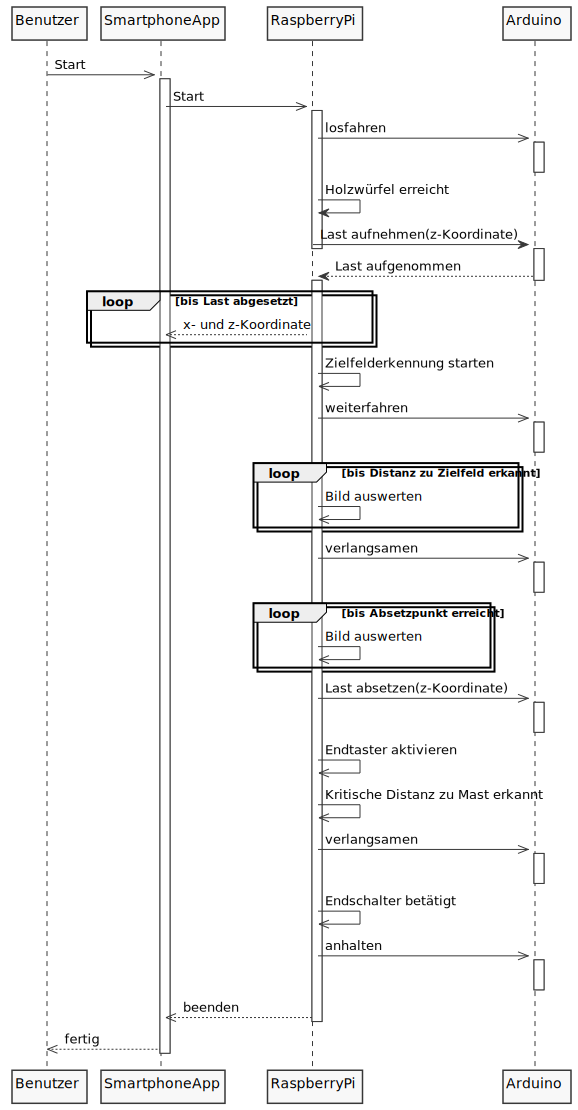
\includegraphics[height=\textheight]{graphs/sequenzdiagramm.png}
    \caption{Die Kommunikation zwischen Benutzer, Smartphone, Raspi und Arduino}
    \label{fig:kommunikation}
\end{figure}

\newpage
\section{Bildverarbeitung}
\label{sec:bildverarbeitung}

Weil das Zielfeld im Gegensatz zum Holzwürfel nicht an einer vorher definierten Stelle auf der x-Achse zu liegen kommt, muss dieses optisch erkannt werden. Hierzu wird, wie in PREN 1 \cite[S. 25-26]{pren1} beschrieben, die Raspi-Cam zusammen mit der Bildverarbeitungsbibliothek OpenCV und der Programmiersprache Python 3 verwendet. Die Herausforderung besteht nicht nur in der Erkennung des Zielfeldes, sondern auch in der Ermittlung der jeweils gegenwärtigen Distanz der Last zum Zielfeld.

\subsection{Lösungsansatz}
\label{sec:loesungsansatz}

Wird die Kamera nach unten zeigend parallel zur Unterlage ausgerichtet, ist der Bildmittelpunkt direkt unterhalb der Kameralinse. Die Distanz von der Kameralinse zum Lastmittelpunkt kann anhand der CAD-Pläne auf ca. $11cm$ festgelegt werden. Dies ist die Distanz, welche die Kamera über das Ziel hinweg positioniert werden muss, um die Last möglichst in der Mitte des Zielfeldes abzulegen.

Die Seitenlänge des innersten Zielfeldquadrates ist in der Aufgabenstellung mit $6cm$ definiert. Dies ist ein wichtiger Referenzwert, anhand dessen der horizontale Abstand zwischen Kameralinse und Zielfeldmittelpunkt ermittelt werden kann.

Die Kamera kann die Seitenlänge des innersten Zielfeldes sowie den Abstand von Bildmitte zum Mittelpunkt des innersten Zielfeldes \textit{in Pixeln} ermitteln. Mit dem Bruch $\frac{\text{ZielfeldhöhePixel}}{6cm}$ kann ermittelt werden, wie vielen Pixeln ein Zentimeter auf dem Bild entspricht. Der horizontale Abstand zwischen Kameralinse und Zielfeldmittelpunkt kann so von Pixeln in eine Distanz in Zentimetern umgerechnet werden.

Dieser Lösungsansatz stellt besondere Anforderungen an die Konstruktion:

\begin{enumerate}
    \item Die Sicht der Kamera nach unten und vorne darf durch kein Bauteil versperrt werden.
    \item Die Kamera muss möglichst parallel zum Untergrund ausgerichtet sein. Seitliche Schwingungen sind unproblematisch, solange das Zielfeld im Sichtfeld bleibt. Starke Schwingungen nach vorne und hinten hingegen lassen das Zielfeld optisch über die gedachte horizontale Bildmittellinie springen, wodurch der hier ausgearbeitete Lösungsansatz nicht mehr funktionieren würde.
\end{enumerate}

Die erarbeitete mechanische Konstruktion erfüllt diese beiden Anforderungen. (Einzig der Blick nach hinten ist von der Greifeinheit versperrt, wodurch zur genauen Positionierung über dem Zielfeld auf den Ultraschallsensor zurückgegriffen werden muss.)

\subsection{Umsetzung}

Die Python-Klasse \texttt{ImageAnalyzer} verfügt über eine Methode namens \texttt{calculate\_distance}, welche von aussen aufzurufen ist. Diese erwartet als Parameter ein Bild als NumPy-Matrix im BGR-Farbraum. Das Bild wird zunächst in Graustufen umgewandelt, indem alle Bildpunkte abhängig von ihrem Helligkeitswert schwarz oder weiss eingefärbt werden.\footnote{Das Zielfeld ist schwarz-grau und nicht schwarz-weiss. In der Praxis trifft man kaum auf ein reines Schwarz oder Weiss.} Das Verfahren wird in \appref{app:thresholding} beschrieben. So wird verhindert, dass feine Linien und Verunreinigungen sowie Klebebänder nicht als Kanten erkannt werden, sondern gleich verschwinden.

Die Polygon-Konturen auf einem Bild können mit der OpenCV-Funktion \texttt{findContours} ermittelt werden. Diese gibt neben einer Liste von Konturmatrizen -- bestehend aus den Koordinaten der Polygonknoten -- die dazugehörigen Polygonhierarchieen zurück. Letztere gibt Auskunft über die Verschachtelungen der ermittelten Polygone.\footnote{Ein Eltern-Polygon beinhaltet ein Kind-Polygon vollständig. Benachbarte Polygone schneiden einander nicht. Das äusserste Polygon einer Hierarchie hat kein Elternpolygon, das innerste Polygon hat kein Kindpolygon.}

Die so ermittelten Polygone müssen genauer untersucht werden, denn es es werden bei weitem mehr gefunden als bloss die konzentrischen Quadrate des Zielfeldes: etwa die gezackten Hindernisse in Form von Tannenattrappen oder die Holzplatten der Unterlage. Diese sollen nach dem Ausschlussverfahren eliminiert werden, indem folgende Heuristiken zum Einsatz kommen:

\begin{description}
    \item[Benachbarte Polygone] Liegen zwei Polygone nebeneinander, bezeichnet man diese als benachbart. Das Zielfeld ist eine Hierarchie von Polygonen, und nur das äusserste Quadrat kann so plausiblerweise einen (oder mehrere) Nachbarn haben. Ein Polygon, das einen Nachbarn hat, ist kein inneres Quadrat des Zielfeldes und kann somit ausgeschlossen werden.
    \item [Quadratische Form] Die zu ermittelnden Polygone sind auf dem Bild nahezu quadratisch, wobei durch perspektivische Verzerrung und Verschwimmen des Bildes (wegen Bewegungsunschärfe) niemals perfekt quadratische Polygone gefunden werden können. Es genügt jedoch Polygone, die nicht einmal näherungsweise ein Quadrat darstellen können, aufgrund zweier Kriterien auszuchliessen:
        \begin{enumerate}
            \item \textsc{Anzahl Ecken}: Ein Quadrat hat vier Ecken. Ein Hindernis, wie die grüne Tannenattrappe ungefähr zwanzig. Polygone mit einer von vier abweichenden Anzahl Knoten können ausgeschlossen werden.
            \item \textsc{Verhältnis Höhe/Breite}: Bei einem Quadrat ist die Höhe gleich der Breite. Bei einem nahezu quadratischen Polygon sollte das Verhältnis $\frac{\text{Höhe}}{\text{Breite}}$ im Bereich $[0.75..1.25]$\footnote{Diese Werte wurden bei Versuchen ermittelt und funktionierten zuverlässig.} liegen.
        \end{enumerate}
    \item[Absolute Grösse] Das innerste Quadrat des Zielfeldes nahm bei Tests immer mehr als 0.5\% der gesamten Bildfläche ein. Das äusserste Quadrat war niemals grösser als 95\% der Bildfläche. Polygone, deren Grösse nicht in dieses Fenster fällt, können ausgeschlossen werden.\footnote{Je nach konfigurierter Vorder- und Hintergrundfarbe kann der Bildrand als Polygon erkannt werden. Die Fläche dieses Polygons beträgt dann 100\% der Bildgrösse.}
\end{description}

Nachdem die Anzahl der gefundenen Polygone nach dem beschriebenen Heuristik-Au\-sschluss\-ver\-fahren reduziert worden ist, bleibt eine Liste von \textit{Kandidaten} übrig, die möglicherweise ein Zielfeld darstellen. Nun gilt es, diese Kandidaten genauer zu untersuchen. Hierzu wird wiederum die Polygonhierarchie verwendet, die schon bei der Ermittlung benachbarter Polygone hilfreich war.

\subsubsection{Die Polygonhierarchie}

Die bereits erwähnte OpenCV-Funktion \texttt{findContours} gibt neben den Polygonkoordinaten auch für jedes Polygon eine Liste bestehend aus vier Zahlen zurück. Die ersten beiden Zahlen handeln von der Nachbarschaftsbeziehung und sind Referenzen auf den Index des vorhergehenden bzw. des nachfolgenden Nachbarpolygons. Da sich in der gefilterten Kandidatenliste keine Polygone mit Nachbarn mehr befinden, können diese Angaben ignoriert werden.\footnote{Sie haben allesamt den Wert \texttt{-1}. Das bedeutet: Kein Nachbar vorhanden.}

Die dritte Zahl gibt den Index des ersten Kindpolygons an. (Da Polygone mit Nachbarn nicht in der Liste vorkommen, gibt es immer nur ein Kindpolygon.) Die vierte Zahl gibt den Index des Elternpolygons an.\footnote{Die Hierarchie-Liste mit vier Elementen ist also als Knoten von gleich zwei verketteten Listen zu verstehen: Einerseits als Element der Nachbarschaftskette und andererseits als Element der Eltern-Kind-Beziehungskette.}

Gesucht ist das \textit{innerste Zielfeld}. Dieses ist definiert als ein Quadrat, das von einem anderen Quadrat umschlossen wird, aber selber keine weiteren Quadrate enthält. Übersetzt auf die Hierarchie-Liste bedeutet das also, dass das dritte Element (erstes Kindpolygon) auf kein anderes Polygon verweisen darf (Wert: \texttt{-1}) und das vierte Element (Elternpolygon) einen gültigen Wert haben muss (Konturindex des jeweiligen Elternpolygons). Wird ein solches Quadrat gefunden, das zuvor schon durch verschiedene Heuristikprüfungen gekommen ist, wird dieses als das innerste Feld des Zielfeldes angenommen. Der Mittelpunkt dieses Polygons wird über die OpenCV-Funktion \texttt{moments} ermittelt.

Wie bereits weiter vorne beschrieben (\secref{sec:loesungsansatz}) kann nun der Abstand zu diesem Zielfeld errechnet werden. Die genaue Positionierung der Last über dem Zielfeld ist im Abschnitt \secrefplain{sec:ablauf} beschrieben.

\subsubsection{Abwägungen}

Die Ermittlung des innersten Zielfeldes könnte noch etwas solider umgesetzt werden, indem nicht nur geprüft wird, ob das innerste Zielfeld \textit{ein} Elternpolygon hat, sondern indem eine \textit{rekursive} Prüfung vorgenommen würde. Das Elternpolygon des innersten Zielfeldes hat wiederum ein Elternpolygon, welches wiederum ein Elternpolygon hat usw. Das vorliegende Zielfeld besteht aus sechs konzentrischen Quadraten, das innerste Zielfeld müsste also fünf übergeordnete Hierarchiestufen besitzen -- und nicht bloss eine. Eine rekursive Prüfung wäre somit solider.

Andererseits bringt eine rekursive Prüfung auch Probleme mit sich:

\begin{description}
    \item[Implementierung] Eine rekursive Prüfung ist aufwändiger umzusetzen und somit fehleranfälliger. Es besteht die Gefahr für Endlosschleifen und somit für einen Stack Overflow, der das Programm zum Abstürzen bringen würde. Das Problem ist zugegebenermassen nicht schwierig zu lösen, und die Endlosschleife könnte mittels Heuristiken vermieden werden. Die Codemenge und -komplexität würde dennoch zunehmen -- und damit auch die Fehlerwahrscheinlichkeit.
    \item[Anzahl Hierarchiestufen] \imgrefplain{fig:zielfeld5} und \imgrefplain{fig:zielfeld6} zeigen das Zielfeld während zweier kurz aufeinanderfolgenden Phasen der Überfahrt. Einmal werden die äusseren beiden Quadrate erkannt, einmal nicht. Dies hat wohl damit zu tun, dass die feine weisse Linie zur Ausrichtung des Zielfeldes auf der x-Achse auf dem etwas verschwommenen Bild den Eindruck macht durchgezogen zu sein. Optisch können keine Quadrate sondern nur halbierte Quadrate (eine andere Art von Polygon mit acht statt vier Ecken) erkannt werden. Die Anzahl der zu prüfenden Hierarchiestufen kann also nicht mit absoluter Sicherheit angegeben werden.
    \item[Früherkennung] Diese beiden genannten Probleme sind sind eher Erschwernisse und Einschränkungen und sollten kein Hindernis für die Umsetzung der rekursiven Hierarchieprüfung darstellen. Aus Gründen der Performance ist die Hierarchieprüfung aber ein grosses Problem. Hierbei geht es nicht etwa um die Programmlaufzeit, sondern um den Zeitpunkt, ab dem das Zielfeld zum ersten mal erkannt werden kann. Ein Blick auf die Bildserie (Seite \pageref{fig:bildserie}) führt dies vor Augen: Auf dem ersten Bild wird noch kein Zielfeld erkannt, da noch kein Quadrat vollständig auf dem Bild sichtbar ist. Auf dem zweiten Bild wird ein Quadrat erkannt.\footnote{Die Bildserie stammt von einem frühen Prototyp der Bildverarbeitung, die alle erkannten Quadrate markiert hat. Mit der Hierarchieprüfung dürfte auf dem zweiten Bild noch kein Zielfeld erkannt werden.} Auf dem dritten Bild werden bereits drei Quadrate erkannt, auf dem vierte Bild sind es bereits fünf Quadrate. Sechs Quadrate werden zum ersten mal auf dem fünften Bild erkannt. Würde die Hierarchie rekursiv geprüft, würde das Zielfeld nicht zum ersten mal mit einem Abstand von $23.4cm$ (\imgrefplain{fig:zielfeld3}) sondern erst mit einem Abstand von $16.3cm$ (\imgrefplain{fig:zielfeld5}) erkannt. \textit{Je tiefer die zu prüfende Hierarchie gewählt wird, desto später wird das Zielfeld erkannt.}
\end{description}

Aus diesen genannten Gründen wurde auf eine \textit{rekursive} Hierarchieprüfung verzichtet. Bei Tests ist bisher nie ein falsches Zielfeld erkannt worden. Die Probleme bestanden eher darin, dass zu Beginn bestimmte Parameter zu streng definiert waren, was später etwas gelockert wurde.

\begin{figure}
    \centering
    \begin{subfigure}{0.3\textwidth}
        \centering
        \includegraphics[width=0.95\linewidth]{pics/zielfeld/01.jpg}
        \caption{noch nichts erkannt}
        \label{fig:zielfeld1}
    \end{subfigure}
    \begin{subfigure}{0.3\textwidth}
        \centering
        \includegraphics[width=0.95\linewidth]{pics/zielfeld/02.jpg}
        \caption{erstes Quadrat}
        \label{fig:zielfeld2}
    \end{subfigure}
    \begin{subfigure}{0.3\textwidth}
        \centering
        \includegraphics[width=0.95\linewidth]{pics/zielfeld/03.jpg}
        \caption{weitere Quadrate}
        \label{fig:zielfeld3}
    \end{subfigure}
    \vskip\baselineskip
    \begin{subfigure}{0.3\textwidth}
        \centering
        \includegraphics[width=0.95\linewidth]{pics/zielfeld/04.jpg}
        \caption{noch mehr Quadrate}
        \label{fig:zielfeld4}
    \end{subfigure}
    \begin{subfigure}{0.3\textwidth}
        \centering
        \includegraphics[width=0.95\linewidth]{pics/zielfeld/05.jpg}
        \caption{sämtliche Quadrate}
        \label{fig:zielfeld5}
    \end{subfigure}
    \begin{subfigure}{0.3\textwidth}
        \centering
        \includegraphics[width=0.95\linewidth]{pics/zielfeld/06.jpg}
        \caption{verschwommene Aufnahme}
        \label{fig:zielfeld6}
    \end{subfigure}
    \vskip\baselineskip
    \begin{subfigure}{0.3\textwidth}
        \centering
        \includegraphics[width=0.95\linewidth]{pics/zielfeld/07.jpg}
        \caption{immer näher}
        \label{fig:zielfeld7}
    \end{subfigure}
    \begin{subfigure}{0.3\textwidth}
        \centering
        \includegraphics[width=0.95\linewidth]{pics/zielfeld/08.jpg}
        \caption{extrem nahe}
        \label{fig:zielfeld8}
    \end{subfigure}
    \begin{subfigure}{0.3\textwidth}
        \centering
        \includegraphics[width=0.95\linewidth]{pics/zielfeld/09.jpg}
        \caption{vorbei}
        \label{fig:zielfeld9}
    \end{subfigure}
    \label{fig:bildserie}
    \caption{Die Bildserie zeigt das Überfahren des Zielfeldes aus Kameraperspektive.}
\end{figure}

\subsection{Auflösung und Verarbeitungsgeschwindigkeit}

Das verwendete Kameramodul \cite{picam} unterstützt eine Bildauflösung von bis zu $3280\times2464$ Bildpunkten, was acht Megapixeln entspricht. Bei den Tests wurden verschiedene Auflösungen ausprobiert, etwa HD-Auflösung ($1080\times1920$ Pixel).\footnote{Die Orientierung der Kamera wird über die Auflösung der Form $\text{Breite}\times\text{Höhe}$ angegeben. Die Auflösung $1920\times1080$ entspricht der HD-Auflösung in \textit{Landscape}-Orientierung (Breitbild), die Auflösung $1080\times1920$ entspricht der HD-Auflösung in \textit{Portrait}-Orientierung (Hochformat). Da das Blickfeld der Kamera möglichst weit nach vorne und nicht in die Breite reichen soll, wird das Hochformat verwendet.} Die besten Ergebnisse wurden mit einer Auflösung von $480\times640$ (VGA-Auflösung) erreicht. Diese geringe Auflösung hat folgende Vorteile:

\begin{description}
    \item[Performance] Das Auswerten von Bildern in HD-Auflösung dauerte ca. $550$ Millisekunden. Mit VGA-Auflösung konnten Bilder in durchschnittlich $45$ Millisekunden ausgewertet werden. Das entspricht einem Performancegewinn von ca. Faktor $12$.
    \item[Unschärfe] Bei der vorliegenden Aufgabe hat sich eine gewisse Unschärfe bei den aufgenommenen Bildern als vorteilhaft erwiesen, da kleinere Konturen, wie etwa Verschmutzungen auf dem Zielfeld und Klebestreifenrückstände auf der Unterlage, bereits bei der Bildaufnahme verschwimmen und so nicht als Konturen erkannt werden. Die scharfen Konturen des Zielfeldes waren bei den Aufnahmen aber dennoch genug scharf.
\end{description}

Für die Testdurchläufe wurden die aufgenommenen Bilder zur späteren Auswertung jeweils abgespeichert. Das Abspeichern der Bilder nahm jeweils ungefähr die Hälfte der Bildverarbeitungszeit in Anspruch: Dauerte die Verarbeitung eines Bildes $45$ Millisekunden, benötigte die Abspeicherung weitere $20$ Millisekunden. Für den Wettbewerb wird das Abspeichern der Bilder aus Performancegründen deaktiviert.

\newpage
\section{Software}

\subsection{Smartphone-App: Java}
\label{sec:smartphoneapp}

Um die autonome Laufkatze zu starten wird eine Smartphone-App verwendet. Dazu muss sich das Smartphone im selben Netzwerk wie der Raspi befinden. Der Raspi übernimmt dabei die Rolle des Servers, und das Smartphone verbindet sich als Client mit ihm. Betätigt der Anwender die Starttaste der App, verbindet sich das Smartphone mit dem Raspi, und die Laufkatze wird gestartet. Sobald die Last aufgenommen wurde, sendet der Raspi fortlaufend die aktuellen Koordinaten der Last an die Smartphone-App. Auf diese Weise sieht der Anwender ununterbrochen die aktuellen Lastkoordinaten auf seinem Smartphone. Dabei zeigt das Smartphone lediglich die empfangenen Koordinaten an und übernimmt keinerlei Logik.

Damit die Kommunikation zwischen Smartphone und Raspi funktioniert, müssen sich beide Geräte im selben Netzwerk befinden. Dazu wird mittels eines \textit{maplite}-Routers ein eigenes Netzwerk mit der SSID \texttt{pren7} aufgebaut. Mit diesem Netzwerk verbinden sich der Raspi und das Smartphone. Damit sich das Smartphone mit dem Raspi verbinden kann, wurde für den Raspi eine statische IP-Adresse konfiguriert.

Für die Entwicklung der Smartphone-App wurde das Android Studio verwendet. Das Android Studio bietet viele Vorteile für die Entwicklung, zum Beispiel einen integrierten Emulator, oder das Debuggen direkt auf dem Smartphone.

\imgrefplain{fig:smartphoneapp} zeigt die Benutzeroberfläche der Smartphone-App.

\begin{figure}[H]
    \centering
    \includegraphics[width=0.25\linewidth]{pics/smartphoneapp.png}
    \caption{Die Smartphone-App zur Steuerung von \textit{Silisloth} und zum Ablesen der Koordinaten}
    \label{fig:smartphoneapp}
\end{figure}

\subsection{Raspi: Python}
\label{sec:raspi}

Die übergeordnete Steuerung und Koordination von \textit{Silisloth} wurde auf dem Raspi mit Python umgesetzt. Der Quellcode zum Projekt findet sich im Anhang (\texttt{silisloth-raspi.zip})

\begin{figure}
    \centering
    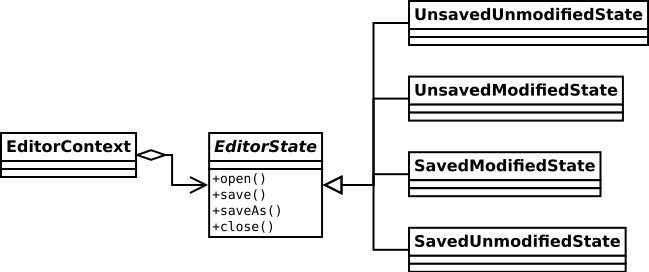
\includegraphics[width=\textwidth]{graphs/klassendiagramm.png}
    \caption{Das Klassendiagramm des Python-Projektes}
    \label{fig:klassendiagramm}
\end{figure}

\subsubsection{Projektstruktur}

Das Projekt besteht aus verschiedenen Quellcodedateien:

\begin{description}
    \item[\texttt{Arduino.py}] Kommunikation mit dem Arduino per serieller Schnittstelle (USB): Die angebotenen Funktionen bieten eine selbsterklärende Schnittstelle für die zu erteilenden und empfangenden Befehle.
    \item[\texttt{Brain.py}] Die übergeordnete Programmlogik: Der ganze Ablauf (\secref{sec:ablauf}) wird von diesem Skript gesteuert.
    \item[\texttt{EndSwitch.py}] Ansteuerung des Mikroendschalters: Es wird eine Funktion zur Verfügung gestellt, die blockierend auf das Betätigen des Mikroendschalters wartet.
    \item[\texttt{ImageAnalyzer.py}] Die Bildverarbeitungslogik: Verarbeitet ein einzelnes Bild und gibt eine Millimeterangabe zurück, die den optischen Abstand in x-Richtung von Kameralinse zum Zielfeldmittelpunkt in Millimetern zurückgibt.
    \item[\texttt{Log.py}] Logger-Konfiguration und -Format für sämtliche im Projekt geschriebenen Logmeldungen: Für die Ausgabe auf den Bildschirm wird aus Gründen der Übersichtlichkeit ein tieferes Log-Level verwendet als für die Ausgabe in die Logdatei.
    \item[\texttt{TargetDetection.py}] Fassade für den \texttt{ImageAnalyzer}: Kümmert sich um die Aufnahme von Bildern und stellt eine vereinfachte Schnittstelle für die Bildverarbeitungslogik und das Abspeichern der aufgenommenen Bildern zu Debug-Zwecken zur Verfügung.
    \item[\texttt{TcpServer.py}] Kommunikation zum Smartphone: Wartet blockierend auf eine eingehende Verbindung und schickt die formatierte Zeichenkette mit den Koordinaten an die Smartphone-App.
    \item[\texttt{UltrasonicSensor.py}] Ansteuerung der Ultraschallsensoren: Bietet Funktionen zur Erstellung von Messreihen. Es kann eine bestimmte Anzahl von Messungen erstellt oder eine bestimmte Zeit lang gemessen werden. Von der Messreihe wird der Median-Wert zurückgegeben, was die Messung robust für Fehlmessungen macht \cite[S. 46-48]{pren1}.
\end{description}

Zum Testen einzelner Komponenten wurden folgende Demo-Programme entwickelt:

\begin{description}
    \item[\texttt{ArduinoMock.py}] Testprogramm für die serielle Kommunikation mit dem Arduino: Befehle können direkt über die Kommandozeile an den Arduino gesendet werden, was zum Testen und zur Fehlersuche hilfreich ist.
    \item[\texttt{ImageAnalyzerDemo.py}] Testprogramm für die Zielfelderkennung: Verarbeitet eine im Dateisystem abgespeicherte Bildserie und gibt die dabei errechneten Abstände vom Zielfeldmittelpunkt auf der Kommandozeile aus.
    \item[\texttt{TargetDetectionDemo.py}] Weiteres Testprogramm für die Zielfelderkennung: Im Gegensatz zur \texttt{ImageAnalyzerDemo} werden die zu verarbeiteten Bilder direkt über die Raspi-Kamera aufgenommen.
    \item[\texttt{UltrasonicDemo.py}] Testprogramm für die Ultraschallsensoren: Es wird eine bestimmte Anzahl von Messungen durchgeführt. Der Median des Messergebnis wird auf die Kommandozeile ausgegeben. Der Vorgang wird endlos wiederholt, womit die Messungen beim manuellen Fahren am Seil überprüft werden können.
\end{description}

\subsubsection{Eingesetzte Python-Bibliotheken}

\begin{description}
    \item[OpenCV] Bildverarbeitungsbibliothek mit Python-Interface \cite{opencv}
    \item[NumPy] Matrizenberechnungen: OpenCV verwendet Matrizen als Datenstruktur für die Bilder \cite{numpy}
    \item[RPi.GPIO] Ansteuerung von GPIO-Ports: Interaktion mit Ultraschallsensoren und dem Mikroendschalter \cite{rpigpio}
    \item[Picamera] Ansteuerung der Raspi-Kamera zur Aufnahme von Bildern \cite{picamera}
    \item[PySerial] Ansteuerung der seriellen Schnittstelle: Kommunikation per USB-Verbindung zum Arduino \cite{pyserial}
\end{description}

\subsection{Arduino: C}

\label{sec:arduino}

Die Motorensteuerung wurde auf dem Arduino umgesetzt. Der Quellcode zum Projekt findet sich im Anhang (\texttt{silisloth-arduino.zip}). Das Projekt ist in folgende Quellcodedateien aufgeteilt:

\begin{description}
    \item[\texttt{Sloth\_Main.ino}] Definition und Initialisierung von globalen Variablen und Tasks.
    \item[\texttt{Sloth\_Communication.ino}] Kommunikation mit dem Raspi per serieller Schnittstelle (\secref{sec:raspi-arduino})
    \item[\texttt{Sloth\_StateMachine.ino}] Die Programmlogik, gemäss einer State-Machine (\imgref{fig:arduino-statemachine})
    \item[\texttt{Sloth\_Functions.ino}] Implementierung diverser Funktionen
\end{description}

Es wurden folgende Arduino-Bibliotheken eingesetzt:

\begin{description}
    \item[Wire] Kommunikation mit I2C
    \item[FreeRTOS] Multitasking (Kommunikation und State-Machine)
    \item[Adafruid\_Motorshield] Ansteuerung von Motoren via Motor Shield
    \item[Utility] PWM

\end{description}

Die State-Machine (\imgref{fig:arduino-statemachine}) gibt Auskunft über die internen Stati und die Befehle, die intern für die Transitionen verwendet wurden.

\begin{figure}
    \centering
    \includegraphics[height=\textheight]{graphs/arduino-statemachine.png}
    \caption{Die State-Machine der Arduino-Lösung}
    \label{fig:arduino-statemachine}
\end{figure}


\newpage
\section{Zielerreichung}
\label{sec:zielerreichung}

Bei der Arbeit an \textit{Silisloth} mussten -- wie die vorliegende Dokumentation zeigt -- viele kleine Details beachtet werden. Es bestand die Gefahr sich in diesen Details und den Blick fürs Ganze zu verlieren. Um dies zu verhindern wurden die einzelnen Komponenten möglichst bald am Prototypen montiert, sodass Tests früh an der «Produktivumgebung» stattfinden mussten, bzw. das Aufbauen eines isolierten Testsettings aufwändiger als ein Test am Prototypen gewesen wäre. Dies förderte zudem die Zusammenarbeit innerhalb der Gruppe, da man sich für Tests immer absprechen musste.

\subsection{Testphase}

Im letzten Drittel des Semesters wurden Tests «am Seil» durchgeführt, wobei das Absolvieren der gestellten Wettbewerbsaufgabe geübt wurde. Diese Tests wurden nicht im Einzelnen protokolliert. Stattdessen ist hier eine Liste mit Erkenntnissen und Verbesserungen aufgeführt, die einen Überblick über den Test- und Lernprozess geben soll:

\begin{description}
    \item[Antriebsmotor] Es stellte sich bald heraus, dass \textit{Silisloth} im Vergleich zu den Prototypen anderer Gruppen sehr langsam fährt. Der zu Beginn verbaute Getriebemotor war eine sehr konservative Wahl: Mit der verbauten Untersetzung hätte er einen weit schwereren Prototypen antreiben können, jedoch nur sehr langsam. Deshalb wurde ein stärkerer Motor verbaut.
    \item[Zielfelderkennung] Die Zielfelderkennung schien bei den ersten Tests bereits perfekt zu funktionieren. Bei geänderten (d.h. dunkleren) Lichtverhältnissen und mit auf dem Zielfeld entstandenen Spuren traten aber plötzlich Probleme auf, die mit kleineren Korrekturen nur scheinbar gelöst werden konnten, indem der Schwarz-Weiss-Schwellwert auf die jeweiligen Lichtverhältnisse optimiert wurde. Da Lichtverhältnisse plötzlich ändern können, wurde in der zweitletzten Woche eine zuverlässigere Lösung mit adaptivem Thresholding erarbeitet, was bei allen Lichtverhältnissen zuverlässig funktioniert.
    \item[Silikongreifer] Der Silikongreifer erforderte einiges an Abstimmungsarbeit. Es wurden verschiedene Versionen mit jeweils kleinen Detailverbesserungen gefertigt, welche sich beim Aufpumpen mehr oder weniger gleichmässig ausdehnten. Beim Greifen der Last mussten die Höhe der Greifeinheit und die Pumpzeit genau eingestellt werden. Auch die Verbindungen zwischen den Luftschläuchen mussten mehrmals überprüft und abgedichtet werden.
    \item[Netzwerk] Zu Beginn der Tests wurden Laptop, Smartphone und Raspi mit dem HSLU-WiFi verbunden. Das Auffinden des Raspi im Netz mittels ARP-Scan dauerte dabei sehr lange. Gegen Ende des Semesters wurde eine eigene Netzwerkumgebung mit dedizierten Geräten (WiFi-Access-Point, Laptop ohne GUI, unpersonalisiertes Smartphone) aufgebaut. Damit konnte sehr schnell getestet werden. Der Austausch mit der Arbeitsumgebung wurde dadurch hingegen etwas erschwert (Übertragen aufgenommener Bilder zur Auswertung, Austausch des Python-Quellcodes). Aus diesem Grund kam die «produktive» Netzwerkumgebung erst in den letzten beiden Wochen zum Einsatz.
    \item[Vorbereitung] An den offiziellen PREN-Terminen (Donnerstag- und Freitagvormittag) musste man oft länger beim Testgelände warten, bis ein Seil frei war. Eine gute Vorbereitung sparte wertvolle Testzeit -- und reduzierte die Wartezeit für andere Gruppen. Dazu gehört, dass die Akkus geladen, die Verbindungen zwischen den involvierten Geräten erstellt, die Steuerprogramme auf Raspi und Arduino aktualisiert und genügend helfende Hände vorhanden sind. Dies funktionierte schon bald so gut, dass bereits nach fünf Minuten Testzeit mehrere Durchläufe absolviert werden konnten.
    \item[Notausschalter] Wurde in einem Testlauf das Zielfeld nicht richtig erkannt, fuhr \textit{Silisloth} ungebremst in den Endpfosten, was zu Beschädigungen an einzelnen Komponenten und an der ganzen Konstruktion hätte führen können. Zu Beginn der Tests wurde in einem solchen Notfall der Akku vom Laststromkreis getrennt, was einige Sekunden dauerte und erheblichen Kraftaufwand benötigte. Darum wurden später zwei Schalter -- je einen für Last- und Steuerstromkreis -- eingebaut, welche bei Bedarf umgelegt werden konnten. So mussten auch vor und nach den Tests keine Kabel mehr ein- bzw. ausgesteckt werden.
\end{description}

\subsection{Beurteilung gemäss Anforderungen}

Die Anforderungsliste (siehe Ordner \texttt{Anhang}) wurde zu Beginn des Projekts festgelegt. Der im Rahmen von PREN 2 erstellte Prototyp soll kritisch darauf geprüft werden, ob er diesen Anforderungen gerecht wird. Dabei werden die Anforderungen in den ersten drei Spalten aufgeführt; in der vierten Spalte wird die Erfüllung der jeweiligen Anforderung gemäss den Tests eingeschätzt. Auf Wunsch- und Unteranforderungen wird dabei nicht eingegangen.

{\footnotesize
\begin{longtable}{|r|p{2cm}|p{5cm}|p{5.5cm}|}
\hline
\textsc{Nr.} & \textsc{Bezeichnung} & \textsc{Details} & \textsc{Einschätzung gemäss Konzept} \\
\hline
    \textsc{1} & \multicolumn{3}{l|}{\textsc{Rahmenbedingungen}} \\
    \hline
    1.1 & Aufbau  & \textit{Silisloth} lässt sich in max. zwei Minuten aufbauen. & Zu zweit in ca. 20 Sekunden möglich \\
    1.2 & Autonomie & \textit{Silisloth} und das I/O-Gerät arbeiten nach dem Startsignal autonom. & Nach Startsignal (per Smartphone-App) kein weiteres Eingreifen nötig \\
    1.3 & Temperaturbe\-reich & Die Geräte sind in einem Temperaturfenster von $0\degree C$ bis $70\degree C$ einsatzfähig. & Keine Temperaturprobleme festgestellt, Schrittmotor und Raspi-CPU mit Kühlkörper ausgestattet \\
1.4 & Lichtverhältnisse & \textit{Silisloth} funktioniert bei $1’000-100’000$ lux. & Probleme bei unterschiedlichen Lichtverhältnissen behoben \\
    1.5 & Zeitrahmen & \textit{Silisloth} erledigt ihre Aufgaben innerhalb von vier Minuten. & Gemessene Zeitdauer: 1 Minute, 7 Sekunden \\
    \hline
    \textsc{2} & \multicolumn{3}{l|}{\textsc{Dimensionen}} \\
    \hline
    2.1 & Länge & max. $480mm$ & $431mm$ (CAD-Modell) \\
    2.2 & Breite & max. $480mm$ & $204mm$ (CAD-Modell) \\
    2.3 & Höhe & max. $580mm$ & $379mm$ (CAD-Modell) \\
    2.4 & Gewicht & max. $7’000g$ Leergewicht & $4'000g$ (CAD-Modell, Herstellerangaben) \\
    \hline
    \textsc{3} & \multicolumn{3}{l|}{\textsc{Antrieb}} \\
    \hline
    3.1 & Höhenüberwin\-dung & \textit{Silisloth} ist in der Lage eine Steigung von max. $40\degree$ zu überwinden. & Höhenüberwindung der Testanlage problemlos ($8.1\degree$) \\
    3.2 & Einsatzbereich & \textit{Silisloth} kann auf einem Seil mit Durchmesser $2-4mm$ montiert werden. & Funktioniert mit Seil der Testanlage \\
3.3 & Ziel & \textit{Silisloth} stoppt nach Berührung des Endpfostens. & Drucktaster meldet Berührung \\
    3.4 & Geschwindigkeit  & \textit{Silisloth} bewegt sich durchschnittlich mit mindestens $15\frac{mm}{s}$. & $20\frac{cm}{s}$ möglich \\
    3.5 & Fahrtrichtung & \textit{Silisloth} ist in der Lage sich vorwärts und rückwärts am Seil zu bewegen. & Vorwärts- und Rückwärtsfahren möglich \\
    \hline
    \textsc{4} & \multicolumn{3}{l|}{\textsc{Lastbeförderung}} \\
    \hline
    4.1 & Greifen & \textit{Silisloth} kann eine quaderförmige Last mit den Kantenlängen von mindestens $45mm$ und höchstens $55mm$ und einem Gewicht von bis zu $200g$ greifen. & Tests mit $50mm$ Kantenlänge und ca. $200g$ Last erfolgreich \\
    4.2 & Heben/Senken  & \textit{Silisloth} kann eine Last von bis zu $200g$ heben und senken. & Bei Tests unproblematisch \\
    4.3 & Abladen & \textit{Silisloth} kann die Last auf dem Zielfeld absetzen. & Luftventile arbeiten schnell und zuverlässig, Greifer löst sich \\
    \hline
    \textsc{5} & \multicolumn{3}{l|}{\textsc{Sensorik}} \\
    \hline
    5.1 & x-Koordinate & Die x-Koordinate muss mit einer Toleranz von $\pm20mm$ bestimmt werden können. & Messgenauigkeit der Ultraschallsensoren: $\pm20mm (>100cm), \pm2.5\%(<100cm)$ \\
    5.2 & z-Koordinate  & Die z-Koordinate muss mit einer Toleranz von $\pm20mm$ bestimmt werden können. & Messgenauigkeit der Ultraschallsensoren: $\pm20mm (>100cm), \pm2.5\%(<100cm)$ \\
5.3 & Zielerkennung  & Das spezifizierte Zielfeld muss mit einer Toleranz von $\pm20mm$ erkannt werden können. & optische Erkennung in diesem Rahmen \\
5.4 & Lasterkennung  & Die Last muss mit einer Toleranz von $\pm$15mm erkannt werden können. & Funktioniert nach Feinabstimmung \\
    \hline
    \textsc{6} & \multicolumn{3}{l|}{\textsc{Kommunikation}} \\
    \hline
6.1 & Startsignal & \textit{Silisloth} empfängt das Startsignal. & Funktioniert per WiFi \\
6.2 & Koordinaten & \textit{Silisloth} sendet die Koordinaten an das Ausgabegerät. &  Funktioniert per WiFi \\
    \hline
    \textsc{7} & \multicolumn{3}{l|}{\textsc{I/O-Gerät}} \\
    \hline
7.1 & Startsignal & Das Gerät sendet beim Start das Signal an \textit{Silisloth}. & Funktioniert per Smartphone-App \\
7.2 & Koordinaten & Das Gerät gibt die x- und z-Koordinaten der Last an. &  Die Koordinaten werden in Abständen von $500ms$ angezeigt \\
    \hline
    \textsc{8} & \multicolumn{3}{l|}{\textsc{Ausnahmebehandlung}} \\
    \hline
    8.1 & Lasterkennung & Falls \textit{Silisloth} den Endpfosten nicht erkennt, soll es durch einen Nothalt beim Berühren des Mastes anhalten. & Drucktaster beendet Ablauf zuverlässig \\
8.2 & Lasterkennung & Falls \textit{Silisloth} die Last nicht erkennt, fährt es automatisch zum Ziel. & Last wird nicht erkannt sondern abgeschätzt, manuelles Not-Aus nötig \\
8.3 & Zielerkennung & \textit{Silisloth} lässt die Last beim Endpfosten fallen, falls es das Zielfeld nicht erkennt. & Drucktaster beendet Ablauf endgültig \\
    8.4 & Schwingen & \textit{Silisloth} hält an, falls die Schwingung in y-Richtung $20\degree$ überschreitet & Nicht umgesetzt, da Schwingungen in y-Richtung unproblematisch \\
8.5 & Lastverlust & \textit{Silisloth} erkennt, wenn es seine Last verliert. & Kann nicht erkannt werden \\
\hline
\caption{Einschätzung der Anforderungserfüllung aufgrund Prototyps \label{tbl:review-anforderungen}}
\end{longtable}
}

Nach Betrachtung von \tblrefplain{tbl:review-anforderungen} kann unterm Strich festgestellt werden, dass sich der Prototyp weitgehend im Rahmen der Anforderungen bewegt. Kleinere Abweichungen, wie etwa die Messungenauigkeit der Ultraschallsensoren bei grosse Distanzen, verursachen keine grösseren Probleme. \textit{Silisloth} kann nicht erkennen, ob die Last nicht aufgenommen oder verloren wurde. Wie auf ein solches Ereignis reagiert werden müsste, wurde nicht konzipiert.

Der Wettbewerb wird zeigen, wie gut die erarbeitete Lösung tatsächlich ist.

\newpage
\section{Rückblick}
\label{sec:schlusswort}

Der Wiedereinstieg nach den kurzen Semesterferien verlief zu Beginn etwas schleppend. Im Bereich Projektmanagement wurde zunächst ein Versuch unternommen mit Jira zu arbeiten, welches den Informatikern aus ihrer Berufspraxis bereits bekannt war. Es stellte sich bald heraus, dass Jira zwar für die Abhandlung von Scrum-Sprints sehr geeignet ist, aber nicht die erwünschten Funktionen für das Projektmanagement bietet. (Ausserdem sind Studentenlizenzen nur für die selbst gehostete Variante von Jira gültig, und die Jira-Lizenzen hätten das Budget bei weitem gesprengt.) So wurde Jira fallengelassen. Das Projekt wurde seither über einfache Aufgabenlisten und mit einem zentralen Projektplan abgewickelt.

Zu Beginn wurde das Projekt in drei Phasen aufgeteilt, wobei zum Ende jeder Phase verschiedene Arten von Tests erfolgreich absolviert werden sollten:

\begin{description}
    \item[1. Phase: Komponenten] Einzelne Komponenten wie Ultraschallensoren, Motoren, Silikongreifer, Luftpumpen etc. wurden isoliert getestet und in ihrer Handhabung verstanden.
    \item[2. Phase: Komponentengruppen] Die erfolgreich getesteten Komponenten wurden zu verschiedenen Komponentengruppen, wie Greifmechanismus, Bildverarbeitung, Distanzmessung etc., kombiniert und zusammen getestet. Hierbei konnte eine Komponente in mehreren Komponentengruppen vorkommen.
    \item[3. Phase: Autonome Laufkatze] Sobald alle Komponentengruppen funktionierten, wurde \textit{Silisloth} komplett montiert und getestet, um so die Wettbewerbssituation zu simulieren.
\end{description}

Zwar gab es mit einzelnen Komponenten im späteren Projektverlauf immer wieder vereinzelte Probleme (z.B. mit ungenauen Ultraschallsensoren, defekten Akkus und gerissenen Silikongreifern), ansonsten konnte dieser Plan aber gut eingehalten werden.

Bei der Maschinentechnik gab es gleich von Beginn an grosse Fortschritte zu verzeichnen. Die CAD-Pläne wurden gegenüber PREN 1 noch etwas verbessert und ergänzt. Die mechanischen Teile waren schnell gefertigt und schon nach wenigen Wochen montiert. In der Semestermitte war \textit{Silisloth} bereits komplett montiert und -- was die Hardware betrifft -- voll einsatzfähig.

Im Bereich Elektrotechnik wurden zu Beginn Versuche mit dem Freedom Board unternommen. Da hier Fortschritte ausblieben, wurde die Entscheidung gefällt auf Arduino umzusteigen. Es stellten sich nun bald erste Erfolge ein, sodass die zu Beginn verlorene Zeit bald aufgeholt werden konnte. Die Schnittstelle zwischen Raspi und Arduino wurde mit der Informatik zusammen definiert und später vereinfacht.

In der Informatik ging es in den ersten Wochen darum ein besseres Verständnis für die Programmiersprache Python 3, die Raspberry-Plattform (v.a. GPIO-Programmierung) und die Bildverarbeitungsbibliothek OpenCV zu erlangen. Mit der bald funktionierenden Zielfelderkennung konnte eines der Hauptprobleme früh aus dem Weg geräumt werden. Weiter wurde auf Basis von alter Hardware eine komplette Testumgebung bestehend aus Smartphone, Laptop und Wireless-Access-Point eingerichtet, um so an der Wettbewerbssituation nicht auf das HSLU-Netzwerk angewiesen zu sein. In der zweiten Semesterhälfte ging es darum die einzelnen Softwarekomponenten zu kombinieren, wobei ein Grossteil von Programmlogik und Parametern während der Tests verbessert wurde.

\subsection{Lessons Learned}

\begin{description}
    \item[Arduino/Freedom Board] Sind auch nach mehreren Wochen kaum Fortschritte zu verzeichnen, befindet man sich wohl auf dem falschen Pfad. Hier hilft es mehr umzudenken als weiter dem Holzweg entlang zu schreiten. Der Wechsel vom Freedom Board auf Arduino führte zu schnellen Fortschritten im Bereich Elektrotechnik.
    \item[Bildverarbeitung] Die Bildverarbeitung war die grösste Hürde im Bereich Informatik. Nach ersten grundlegenden Funktionstests in PREN 1 ist diese Komponente aber recht lange liegen geblieben. Doch schon nach kurzer (wenn auch intensiver) Beschäftigung mit der Bildverarbeitung im ersten Drittel von PREN 2 konnte eine solide Lösung ausgearbeitet werden. Desto länger man eine schwierige Aufgabe herausschiebt, desto schwieriger und bedrohlicher wirkt sie. Darum ist es wichtig, heikle Aufgaben sofort anzugehen, auch wenn ein schneller Erfolg nicht in Aussicht steht. Durch kleine, inkrementelle Verbesserungen verliert die ungelöste Aufgabe ihr Bedrohliches.
    \item[Multithreading] Python unterstützt die wirklich parallele Ausführung von Programmlogik nur über separate Prozesse, nicht über Threads \cite[S. 122]{effective-python}. Es dauert aber länger einen Prozess aufzustarten als einen Thread. Ausserdem ist die Kommunikation zwischen verschiedenen Prozessen verglichen mit Threads nur mit grossen Einschränkungen möglich. Die Idee, die vier Prozessorkerne des Raspi mit paralleler Ausführung von Programmlogik auszunützen, musste bald verworfen werden. Die Kommunikation vom Raspi zur Smartphone-App bzw. zum Arduino war anfänglich auch mit Threads gelöst. Dies führte zunächst bei den Messungen mit den Ultraschallsensoren zu Problemen, welche später mit fehleranfälligem Synchronisationscode teilweise gelöst wurden. Im weiteren Verlauf wurden Programmlogik und Kommunikationsprotokoll soweit vereinfacht, dass schliesslich ganz auf Threads verzichtet werden konnte. Ein Programmierproblem sollte zunächst so einfach wie möglich gelöst werden. Über die Ausführungsgeschwindigkeit sollte man sich erst dann Gedanken machen, wenn sie sich als ungenügend herausstellt.
    \item[Race Conditions] Im Gegensatz zum Raspi wurden auf dem Arduino mehrere Threads ausgeführt. Einer kümmerte sich um die Kommunikation mit dem Raspi (Kommunikationsthread), der andere regelte die Motoren (Koordinationsthread). Beim Erteilen des \texttt{Sxxx;}-Signals zum Herablassen der Greifeinheit traten dabei Probleme auf, da der Arduino den Befehl ignorierte. Es stellte sich heraus, dass der Arduino das Zeichen \texttt{S} über den Kommunikationsthread erhielt, der Koordinationsthread aber vor dem Einlesen der Anzahl Millimeter nicht in den entsprechenden Status wechselte, da in der Zwischenzeit kein Kontextwechsel stattfand. Es lag also eine klassische \textit{Race Condition} vor! Das Problem wurde gelöst, indem der Kommunikationsthread nach Erhalt des Zeichens \texttt{S} selber den Statuswechsel vornahm, sodass die darauf übertragene Zahl korrekt eingelesen und ausgewertet werden konnte. Bei Threads darf man keine Annahmen über Kontextwechsel treffen!
    \item[Entladen von LiPo-Akkus] Werden LiPo-Akkus (oder einzelne Batteriezellen) zu stark entladen, sodass die Spannung unter $3V$ fällt, gilt der Akku als beschädigt und kann nicht mehr aufgeladen werden. Dies ist während Tests einmal geschehen, wonach die Testserie unterbrochen, sowie ein neuer Akku angeschafft werden musste. Dies hat nicht nur Geld sondern auch wertvolle Testzeit gekostet. Deshalb wurde mit dem neuen LiPo-Akku sogleich ein \textit{LiPo-Checker} angeschafft: ein kleines elektronisches Bauteil, das an den LiPo-Akku angeschlossen wird und mit einer grünen und roten LED den Ladestatus jeder Zelle darstellt. Fällt die Spannung bis zu einem kritischen Bereich ab, erzeugt der LiPo-Checker einen ohrenbetäubenden Lärm, sodass man den Akku sofort aussteckt und nicht länger betreibt. Für den kleineren LiPo-Akku, der den Raspi speist, ist das Problem weniger gravierend, da ein Spannungsabfall vorher durch das Herunterfahren des Betriebssystems bemerkt wird. Der Akku sollte dennoch nach den Testläufen von der USV getrennt werden, da eine LED auch Strom verbraucht und so den Akku entlädt.
\end{description}

\subsection{Fazit}

Die Arbeit an \textit{Silisloth} begann Mitte September 2017 und dauerte bis Juni 2018 an, wobei das Projekt im Januar und Februar 2018 ruhte. Gab es vor neun Monaten nur einen Projektauftrag und eine (anfangs unvollständige) Liste von Gruppenmitgliedern, gibt es jetzt eine voll funktionsfähige autonome Laufkatze namens \textit{Silisloth} und ein Team, das gut zusammengewachsen ist und alle Herausforderungen erfolgreich meistern konnte.
Um ein abschliessendes Fazit zu ziehen lohnt sich der Vergleich mit den Zielen, die sich das Team selber im letzten September gegeben hat \cite[S. 49]{pren1}.

\subsubsection{Gruppenziele}

\begin{description}
\item[Ziel 1] \textit{Wir wollen gut zusammen arbeiten -- auch über die Fachbereiche hinweg.}

Die Zusammenarbeit über das ganze Team hinweg hat während des ganzen Projekts gut funktioniert. Es gab viele Diskussionen, aber keinen Streit. Probleme und Meinungsverschiedenheiten konnten unkompliziert gelöst werden.

\item[Ziel 2] \textit{Wir wollen Spass an der Arbeit haben.}

Das Projekt war sehr motivierend und hat den Gruppenmitgliedern nicht nur viel Arbeit beschert, sondern auch Freude bereitet. Für Tests wurde auch Freizeit geopfert.

\item[Ziel 3] \textit{Wir wollen etwas lernen -- in unserem Fachbereich und fachbereichübergreifend.}

Die Gruppe war in den drei Fachbereichen Maschinentechnik, Elektrotechnik und Informatik gut besetzt, sodass niemand im Fachbereich der anderen eingreifen musste. Wo gegenseitige Hilfe über die Fachgrenzen hinweg möglich war, wurde diese geleistet. Es ist nicht so wichtig, in den für einen fremden Fachbereichen etwas zu leisten, sondern die Perspektive der anderen Fachbereiche einzunehmen, um eine gute Zusammenarbeit zu ermöglichen. Spezialisten dürfen Spezialisten sein, solange sie zu einem Perspektivwechsel fähig sind.

\item[Ziel 4] \textit{Wir wollen, dass jedes Gruppenmitglied seinen Beitrag leistet.}

Bei den sehr vielfältigen Tätigkeiten -- Konzeption, Planung, Recherche, Berechnung, Fertigung, Montage, Messung, Beschaffung, Programmierung, Testen, Projektplanung, Dokumentation, Netzwerkverwaltung, Konfiguration usw. usf. -- konnte sich jedes Teammitglied einbringen und einen Beitrag leisten.

\item[Ziel 5] \textit{Wir wollen eine sichere, zuverlässige und für alle verständliche Lösung erarbeiten, nicht den Wettbewerb um jeden Preis gewinnen.}

Zwar versteht nicht jedes Gruppenmitglied die Details der gesamten Lösung. Dennoch kann jeder Auskunft darüber geben, welches Problem mit welchen Komponenten gelöst wurde, wie diese grob funktionieren, und die Entscheidungen dahinter nachvollziehen.

Die gefundene Lösung arbeitet zwar langsamer als andere Prototypen, dafür sehr zuverlässig und genau. Was beim Wettbewerb drin liegt, wird sich zeigen.
\end{description}

\newpage
\pagestyle{plain}
\appendix

\section{Anhang}
\label{app:anhang}

\subsection{Kostenübersicht}

\tblrefplain{tbl:kostenbudget} gibt Auskunft darüber, wie das Budget von CHF $500.00$ in PREN 1 und PREN 2 verwendet wurde.

\begin{table}
    \footnotesize
    \centering
    \begin{tabular}{l|l|l|r|r|r}
        & \textsc{Artikel} & \textsc{Bereich} & \textsc{Stk.} & \textsc{Preis} & \textsc{Summe} \\
        \hline
        \multirow{11}{*}{\begin{turn}{90}\textsc{PREN 1}\end{turn}}
            & Silikon & Greifeinheit & $0.50$ & $71.90$ & $35.95$ \\
            & Luftpumpe & Greifeinheit & $2.00$ & $1.95$ & $3.90$ \\
            & Raspberry Pi & Steuerung & $1.00$ & $39.90$ & $39.90$ \\
            & Raspi-Cam & Zielfelderkennung & $1.00$ & $29.90$ & $29.90 $ \\
            & SD-Karte $16 GB$ & Steuerung & $1.00$ & $19.90$ & $19.90$ \\
            & Arduino Uno & Steuerung & $1.00$ & $25.00$ & $25.00$ \\
            & Motor Shield & Steuerung & $1.00$ & $6.95$ & $6.95$ \\
            & LiPo-Akku $3000mAh/3.7V$ & Stromversorgung & $1.00$ & $19.90$ & $19.90$ \\
            & Adafruit Power-Boost (USV) & Stromversorgung & $1.00$ & $27.90$ & $27.90$ \\
            & Netzteil & Stromversorgung & $1.00$ & $10.00$ & $10.00$ \\
            & \textsc{Zwischentotal} & & & & $\boldsymbol{219.30}$ \\
            \hline
        \multirow{24}{*}{\begin{turn}{90}\textsc{PREN 2}\end{turn}}
            & Zahnriemen & Hubmechanismus & $1.00$ & $6.95$ & $6.95$ \\
            & Riemenrad klein & Hubmechanismus & $1.00$ & $10.95$ & $10.95$ \\
            & Riemenrad gross & Hubmechanismus & $1.00$ & $12.95$ & $12.95$ \\
            & Angelschnur & Hubmechanismus & $1.00$ & $9.90$ & $9.90$ \\
            & Schrittmotor & Hubmechanismus & $1.00$ & $14.05$ & $14.05$ \\
            & Kugellager & Antrieb & $2.00$ & $4.15$ & $8.30$ \\
            & Getriebemotor 1:50 & Antrieb & $1.00$ & $29.45$ & $29.45$ \\
            & Getriebemotor & Antrieb & $1.00$ & $24.95$ & $24.95$ \\
            & Riemenrad klein & Antrieb & $2.00$ & $12.95$ & $25.90$ \\
            & Magnetventil & Greifeinheit & $1.00$ & $4.80$ & $4.80$ \\
            & Spiralkabel & Greifeinheit & $1.00$ & $5.80$ & $5.80$ \\
            & Silikon & Greifeinheit & $0.50$ & $71.90$ & $35.95$ \\
            & Quick-Pins & Aufhängung & $2.00$ & $2.50$ & $5.00$ \\
            & Motor Shield & Steuerung & $1.00$ & $18.75$ & $18.75$ \\
            & DC-Konverter & Schaltung & $1.00$ & $5.95$ & $5.95$ \\
            & USB-Kabel A-Micro-A & Schaltung & $1.00$ & $7.45$ & $7.45$ \\
            & USB-Kabel A-B & Schaltung & $1.00$ & $9.45$ & $9.45$ \\
            & Prüfsummer & Schaltung & $1.00$ & $10.95$ & $10.95$ \\
            & Relais & Schaltung & $1.00$ & $3.45$ & $3.45$ \\
            & Ultraschallsensor & Sensorik & $2.00$ & $3.71$ & $7.42$ \\
            & LiPo-Akku $1300mAh/14.8V$ & Stromversorgung & $1.00$ & $27.45$ & $27.45$ \\
            & Kleinteile, Diverses & Fertigung & $1.00$ & $30.00$ & $30.00$ \\
            & Holz, Haken, Seil etc. & Gestell & $1.00$ & $24.10$ & $24.10$ \\
            & \textsc{Zwischentotal} & & & & $\boldsymbol{339.92}$ \\
            \hline
        & \textsc{Gesamttotal} & & & & $\boldsymbol{559.22}$
    \end{tabular}
    \caption{Das Kostenbudget für PREN 1 und PREN 2\label{tbl:kostenbudget}}
\end{table}

\subsection{Thresholding-Benchmarks}
\label{app:thresholding}

Um die verschiedenen Thresholding-Verfahren bei unterschiedlichen Lichtverhältnissen zu erproben, wurden zwei Bildserien verwendet. \footnote{Die Helligkeit ist nicht von der Kamera abhängig. Die Bildserien wurden an verschiedenen Tagen aufgenommen, wobei der Raum einmal mit den Storen verdunkelt und das andere mal von Sonnenlicht durchflutet war.}

\begin{enumerate}
    \item Bildserie
        \begin{itemize}
            \item Kamera: Raspi-Cam
            \item Auflösung: $480 \times 640$
            \item zu erkennende Zielfelder: 13
            \item Lichtverhältnisse: eher dunkel, Kunstlicht
        \end{itemize}
    \item Bildserie
        \begin{itemize}
            \item Kamera: Smartphone-Kamera 
            \item Auflösung: $1920 \times 2560$
            \item zu erkennende Zielfelder: 18
            \item Lichtverhältnisse: eher hell, Sonnenlicht
        \end{itemize}
\end{enumerate}

Zu Beginn wurde nur das statische Thresholding-Verfahren implementiert. Beim Simulieren der Wettbewerbssituation kam es dabei immer wieder zu Unregelmässigkeiten: einmal funktionierte die Zielfelderkennung, einmal nicht. Dieser Umstand konnte auf Verschmutzungen und Beschädigungen am verwendeten Zielfeld zurückgeführt werden. Mit der Anpassung des absoluten Threshold-Wertes konnte das Zielfeld wieder erkannt werden. Diese Korrektur führte jedoch dazu, dass Tests an anderen Tagen und -- wie es sich herausstellte -- bei anderen Lichtverhältnissen erneut fehlschlugen.

Aus diesem Grund wurde ein adaptives Thresholding-Verfahren erprobt. Dabei wird das Bild nicht anhand eines fixen Wertes in Graustufen umgewandelt -- ist ein Pixel heller als $x$ wird er weiss, sonst schwarz. Stattdessen wird die Umgebung eines Pixels auf dessen Helligkeitsverteilung analysiert, und die dabei ermittelte Verteilung als Entscheidungsgrundlage für das Einfärben verwendet. Die Grösse der Umgebung hat sich dabei als kritischer Parameter herausgestellt und wurde mit $1/4$ der Bildgrösse sehr gross gewählt, was sich positiv auf das Erkennungsergebnis, jedoch negativ auf die Performance auswirkte (\tblref{tbl:thresholding} -- die Werte $100$, $110$, $120$ bei den statischen Verfahren beziehen sich auf den gewählten absoluten Threshold-Wert im Bereich von $0$: schwarz bis $255$: weiss).

\begin{table}
    {\small
    \begin{tabularx}{\textwidth}{l|r|r|r|r|r|r}
        & \multicolumn{3}{l|}{\textsc{1. Bildserie}} & \multicolumn{3}{l}{\textsc{2. Bildserie}} \\
        \hline
        \textsc{Verfahren} & Erkannt & Zeit (Mean) & Zeit (Median) & Erkannt & Zeit (Mean) & Zeit (Median) \\
        \hline
        Statisch ($100$) & $11/13$ & $35ms$ & $36ms$ & $11/18$ & $354ms$ & $355ms$ \\
        \hline
        Statisch ($110$) & $7/13$ & $36ms$ & $36ms$ & $18/18$ & $348ms$ & $346ms$ \\
        \hline
        Statisch ($120$) & $1/13$ & $34ms$ & $34ms$ & $18/18$ & $355ms$ & $355ms$ \\
        \hline
        Adaptiv (Gauss) & $13/13$ & $333ms$ & $334ms$ & $18/18$ & $77499ms$ & $77520ms$ \\
        \hline
        Adaptiv (Mean) & $13/13$ & $46ms$ & $47ms$ & $18/18$ & $552ms$ & $553ms$ \\
        \hline
    \end{tabularx}
    }
    \caption{Die Benchmarking-Ergebnisse der verschiedenen Thresholding-Verfahren}
    \label{tbl:thresholding}
\end{table}

Aus den Thresholding-Benchmarks\footnote{Die Benchmarks wurden auf einem Raspberry Pi 3 Modell B durchgeführt.} wurden folgende Erkenntnisse gewonnen:

\begin{itemize}
    \item Das statische Verfahren ist performanter als das adaptive.
    \item Bei den statischen Verfahren konnte kein Threshold gefunden werden, mit dem alle Zielfelder erkannt werden können. Der Threshold müsste an die Lichtverhältnisse angepasst werden.\footnote{Bei Sonneneinstrahlung ändern sich die Lichtverhältnisse in Sekunden, wenn eine Wolke die Sonne verdeckt.} Das statische Verfahren ist somit unsicher.
    \item Bei den adaptiven Verfahren konnten alle Zielfelder erkannt werden.
    \item Das Gauss-Verfahren ist um ca. Faktor $7$ (geringe Auflösung) bzw. $140$ (hohe Auflösung) langsamer als das Mean-Verfahren.\footnote{Die Laufzeit wächst etwas schneller als linear zur Auflösung.}
    \item Für kleine Auflösungen beträgt die Performance-Einbusse mit dem Adaptiv-Mean-Verfahren gegenüber den statischen Verfahren ca. $30\%$. Diese Performance ist immer noch wettbewerbstauglich.
\end{itemize}

\textsc{Fazit}: Das Adaptiv-Mean-Verfahren (in Kombination mit einer Auflösung von $480 \times 640$ Pixeln) kommt zum Einsatz. Dieses ist zwar etwas langsamer als das statische Verfahren, arbeitet aber bei allen erprobten Lichtverhältnissen fehlerfrei.\footnote{Ein fehlerhafter Algorithmus kann mit beliebig hoher Performance implementiert werden, sogar mit $O(0)$.}

\subsection{Weitere}

Im Verzeichnis \texttt{Anhang} befinden sich folgende Anhänge:

\begin{description}
    \item[\texttt{Dokumentation\_PREN-1.pdf}] Das \textit{Silisloth}-Konzept aus PREN 1, auf welches in der vorliegenden Arbeit oft verwiesen wurde.
    \item[\texttt{Anforderungsliste\_PREN-1.pdf}] Die Anforderungen aus PREN 1, welchen \textit{Silisloth} genügen sollte.
    \item[\texttt{Assembly-Zeichnungen.pdf}] Das CAD-Modell für \textit{Silisloth} aus verschiedenen Perspektiven.
    \item[\texttt{silisloth-app.zip}] Der Quellcode zur Smartphone-App (Java).
    \item[\texttt{silisloth-raspi.zip}] Der Quellcode zum Raspi-Projekt (Python).
    \item[\texttt{silisloth-arduino.zip}] Der Quellcode zum Arduino-Projekt (C).
\end{description}

\newpage
\bibliographystyle{apacite}
\bibliography{dokumentation}
\newpage
\listoffigures
\addcontentsline{toc}{section}{Abbildungsverzeichnis}
\newpage
\listoftables
\addcontentsline{toc}{section}{Tabellenverzeichnis}

\end{document}
